\documentclass[letterpaper,12pt]{report}
\usepackage{cuproposal}
\usepackage{mathtools}
\usepackage{graphics} % for pdf, bitmapped graphics files
\usepackage{graphicx}
\usepackage{multicol} % man ezafe kardam
%\usepackage{subfigure}
\usepackage{caption}
\usepackage{subcaption} % man ezafe kardam
\usepackage{url}
\usepackage{array}
\usepackage[letterpaper, left=1.4in, right=1.15in, bottom=1.2in, top=0.8in, nohead]{geometry}
\usepackage{mathptmx} %  assumes new font selection scheme installed
\usepackage{amsmath}  %  assumes amsmath package installed
\usepackage{amssymb}  %  assumes amsmath package installed
\usepackage{varioref} %  smart page, figure, table, and equation referencing
\usepackage{fancyvrb} %  extended verbatim environments
\fvset{fontsize=\footnotesize,xleftmargin=2em}
\usepackage{amsthm}
\usepackage{multirow}
\usepackage{verbatim}
\usepackage{mathrsfs}
\usepackage[mathcal]{euscript}
\usepackage{cases}
\usepackage{xtab}
\usepackage{float}    % Used to put figures exactly 'here' in text [h]
\usepackage{dsfont}
\usepackage{enumitem}
\usepackage[export]{adjustbox}
\usepackage[utf8]{inputenc}
\usepackage{lmodern} % changes the font to modern style
\usepackage[T1]{fontenc}
\usepackage{hyperref}
\usepackage{cite}
\usepackage{color}
\usepackage{xcolor}
\definecolor{nicered}{rgb}{0.8,0.1,0.3}
\definecolor{niceblue}{rgb}{0.1,0.1,0.8}
\renewcommand{\citeleft}{\textcolor{nicered}{[}}
\renewcommand{\citeright}{\textcolor{nicered}{]}}
\hypersetup{
    colorlinks=true,
    linkcolor = niceblue,
    citecolor=nicered,
}
\usepackage{arydshln}
\usepackage{leftidx}
\usepackage{blkarray}
\newcommand{\mx}[1]{\mbox{\scriptsize#1}}% Matrix index
\usepackage{lipsum}
\usepackage{enumitem}
\setlist[enumerate]{itemsep=0mm}
\usepackage{booktabs}
\usepackage{siunitx}

%\usepackage[bottom]{footmisc} % keeps footnotes at the bottom
%\usepackage{endnotes}
%\let\footnote=\endnote
\usepackage{makecell} % for bold horizontal line
%\usepackage[math]{cellspace}



%%%%%%%
%%%%%%% For Algorithm2e and coloring box
%#################Start for making Colouful Box in Algorithm
\usepackage{tikz}
\usetikzlibrary{calc,fit}

% code by Andrew Stacey
% http://tex.stackexchange.com/a/50054/3954    
\makeatletter
\tikzset{%
  remember picture with id/.style={%
    remember picture,
    overlay,
    save picture id=#1,
  },
  save picture id/.code={%
    \edef\pgf@temp{#1}%
    \immediate\write\pgfutil@auxout{%
      \noexpand\savepointas{\pgf@temp}{\pgfpictureid}}%
  },
  if picture id/.code args={#1#2#3}{%
    \@ifundefined{save@pt@#1}{%
      \pgfkeysalso{#3}%
    }{
      \pgfkeysalso{#2}%
    }
  }
}

\def\savepointas#1#2{%
  \expandafter\gdef\csname save@pt@#1\endcsname{#2}%
}

\def\tmk@labeldef#1,#2\@nil{%
  \def\tmk@label{#1}%
  \def\tmk@def{#2}%
}

\tikzdeclarecoordinatesystem{pic}{%
  \pgfutil@in@,{#1}%
  \ifpgfutil@in@%
    \tmk@labeldef#1\@nil
  \else
    \tmk@labeldef#1,(0pt,0pt)\@nil
  \fi
  \@ifundefined{save@pt@\tmk@label}{%
    \tikz@scan@one@point\pgfutil@firstofone\tmk@def
  }{%
  \pgfsys@getposition{\csname save@pt@\tmk@label\endcsname}\save@orig@pic%
  \pgfsys@getposition{\pgfpictureid}\save@this@pic%
  \pgf@process{\pgfpointorigin\save@this@pic}%
  \pgf@xa=\pgf@x
  \pgf@ya=\pgf@y
  \pgf@process{\pgfpointorigin\save@orig@pic}%
  \advance\pgf@x by -\pgf@xa
  \advance\pgf@y by -\pgf@ya
  }%
}
\newcommand\tikzmark[2][]{%
\tikz[remember picture with id=#2] #1;}
\makeatother
% end of code by Andrew Stacey

\newcommand\MyBox[4][-1ex]{%
  \tikz[remember picture,overlay,pin distance=0cm]
  {\draw[draw=#4,line width=1pt,fill=#4!20,rectangle,rounded corners]
( $ (pic cs:#2) + (-1ex,2ex) $ ) rectangle ( $ (pic cs:#3) + (1ex,#1) $ );
}
}
%#################End for making Colouful Box in Algorithm

%==========================================
% Algorithm2e
\usepackage[algo2e,ruled,vlined,linesnumbered] {algorithm2e}
\LinesNumbered
\DontPrintSemicolon
\SetAlFnt{\scriptsize}
\SetAlCapFnt{\scriptsize}
\SetAlCapNameFnt{\scriptsize}
\SetAlTitleFnt{\scriptsize}
\SetAlgoNlRelativeSize{-1}  % algo lines numbers 1 level smaller than algo text
                            % norelsize: no change to linenumber size (manual)
\usepackage{xcolor}
% \definecolor{lightgray}{gray}{0.9}
\newcommand\mycommfont[1]{\tiny\sffamily\bfseries\textcolor{blue}{#1}}
\SetCommentSty{mycommfont}
% %%%%%%%%%%%%%%%%%%%%%%%%%%%%%%%%%%%%%%%%
%%%%%%%
%%%%%%%



\begin{document}


\cutitle{An Anomaly Detection System based on Ensemble of Detectors with Effective Pruning Techniques}

\cudept{Electrical and Computer Engineering}
\cudegree{Master of Applied Science}
\cudegreeshort{M.A.Sc.}
\cufname{Amirreza}
\culname{Soudi}
\cumonth{December}
\cuyear{2015}

\cuchair{Dr. VVVVVVVVV}
\cuextexaminer{Dr. XXXXXX , Examiner, External}
\cuexaminerA{Dr. YYYYYYY, Examiner}
\cusupervisor{Dr. ZZZZZZZZ, Supervisor}
\cucosupervisor{Dr. WWWWWWW, Supervisor}

\cuabstract{Anomaly detection systems are important tools for security. Unlike signature-based systems, anomaly detection can be used to detect new attacks for which signatures are now available.

To this end, anomaly detection techniques rely on machine learning techniques to model the normal behaviour of the system. This model is used as a baseline for the detection of anomalies during system operation.

The problem is that there is no one machine learning technique that can provide good accuracy. What we need is to combine multiple techniques. This is because ensemble methods have been used to improve the overall detection accuracy in traditional machine learning. 

The combination consists of combining the outputs of several accurate and diverse models. To reduce the number of combination, and hence improve the efficiency of combination, in this thesis, we propose PBC (Pruning Boolean Combination), an efficient approach for selecting and combining anomaly detectors. PBC relies on two novel pruning techniques that we have developed to  prune redundant and trivial detectors. Compared to existing work, PBC reduces significantly the number of detectors to combine, while keeping similar accuracy. We show the effectiveness of PBC when applying it to benchmarks data sets.

Much of the content of this thesis is adapted and expanded from a paper published at the 2015 IEEE International Conference on Software Quality, Reliability and Security (QRS). QRS is a merger of the SERE conference (IEEE International Conference on Software Security and Reliability) and the QSIC conference (IEEE International Conference on Quality Software)~\cite{Soudi2015}. 
}
\cudedication{{\it Dedicated to

\begin{center}
My Family
\end{center}
}
}
\cuthanks{I owe my deepest gratitude to my beloved family, whose
boundless love and continuous encouragement was unremitting source of inspiration
for this work, specially my sister Afsoon who helped me a lot by all means in the past couple of years.  No words can express how grateful I am for your love and support and
how much I love and appreciate you.

My deepest gratitude is to my supervisor, Dr. Abdelwahab Hamou-Lhadj. I have been amazingly fortunate to have a supervisor who gave me the freedom to explore on my own, and at the same time the guidance to recover when my steps faltered. His patience and support helped me overcome many crisis situations and finish this thesis. I am grateful to him for holding me to a high research standard and enforcing strict validations for each research result.

Beside I owe a dept of gratitude to my supervisor's postdoctoral fellow, Dr. Wael Khreich, who has been always there to listen and give advice. I am deeply grateful to him for the long discussions that helped me sort out the technical details of my work. 

Many friends have helped me stay sane through these difficult years. I greatly value their friendship and I deeply appreciate their belief in me. Special thanks to Ali Sehizadeh, not only for helping me through my master, but also for being warm hearted friends. I should have my special thank to my friends whose friendship going back to my bachelor days, thank you to the supportive friend Afshin Moazami.
Special thanks to Elnaz Davoodi and Nassim Masoudifar, for encouraging me along the way.
I am also indebted to my friends, Yashar Zeighami, Masoud Karzand, Pouya jabbari and Majid Laali for their support, comments and feedback.

I would also like to deeply thank DRDC (Defence R\&D Canada), Ericsson, NSERC (Natural Sciences and Engineering Research Council of Canada), and the Faculty of Engineering and Computer Science at Concordia University for their financial support. This work would not have been possible without them.

Additionally, I would like to thank all members of the Software Behaviour Analysis (SBA) Research Lab at ECE, Concordia for their friendship and encouragement. They brought the perfect atmosphere to combine work and life.

}

\cumaketitlepage
\cumakesignaturepage
\dsp
\cumakeabstract
\cumakededication
\dsp
\cumakethanks
\cutocdeep{2}          % how deep you want to go in the toc: 0: reset to 1
%% and align section with chapter, check to see.
% 1: chap+sec (section indented),
% 2: chap+sec+subsec ...
% the default is now 2.  previously it was 0.
\cumaketableofcontents % Guess,
%\addcontentsline{toc}{chapter}{List of Figures}
\cumakelistoffigures   % id.
%\addcontentsline{toc}{chapter}{List of Tables}
\cumakelistoftables    % id.
%\addcontentsline{toc}{chapter}{}
%\culistofsymbols
%{

\begin{center}
\tabletail{\hline}
	\begin{tabular}{    p{3.0cm}  p{11cm} }
	\multicolumn{2}{c}{\textbf{List of Symbols}} \\	\hline \hline
	        $f$	   		    &	Frequency,~Hz\\
            $\omega$	    &   Angular frequency,~rad/s\\
            $f_s$	 	    &	Sampling frequency\\
            $T_{rec}$	    &	Record time\\
            $T_{win}$	    &	Window length\\
            $G_{uu}$	    &	Input autospectrum\\
            $G_{zz}$	    &   Output autospectrum\\
            $G_{uz}$	    &	Input-output cross-spectrum\\
            $\varepsilon_r$	    &	Random error estimate\\
            $\gamma^2$	    &   Coherence function\\     
            $\tilde{H}~\hat{H}~\hat{H}_c$	    & Rough, smooth, and composite frequency-response estimates\\ \hline
            $u~v~w$	    &	Translational velocities \\
            $p~q~r$	    &	Angular rates\\ 
            $\phi~\theta~\psi$	    &	Euler angles\\ 
            $X~Y~Z$	    &	Aerodynamic forces\\ 
            $L~M~N$	    &	Aerodynamic moments\\    
            $\delta_{lon}~\delta_{lat}~\delta_{col}~\delta_{ped}$	    &	Control inputs\\    
            $I_{xx}~I_{yy}~I_{zz}$	    &	Moments of inertia\\   \hline 
            $J$	    &	Cost function\\
            $\boldsymbol{\theta}$	    &	Vector of unknown parameters\\    
            $\boldsymbol{M}$	    &	Hessian matrix\\
            $\boldsymbol{S}$	    &	Sensitivity matrix\\    \hline
            $\Re$	    &	Real part of a complex number\\ 
            $\dagger$	    & Complex conjugate transpose	
	\end{tabular}%	}
\end{center}



\begin{center}
\tabletail{\hline}
	\begin{tabular}{    p{3.0cm}  p{9cm} }
	\multicolumn{2}{c}{\textbf{Abbreviations and Acronyms}} \\ \hline \hline
         UAV	&	Unmanned Aerial Vehicle\\
         SID   	&	System IDentification \\
         SISO  	&	Single Input/Single Output\\
         MIMO  	&	Multiple Input/Multiple Output\\
         R/C   	&	Radio-Controlled\\
         PIC	&	Pilot In Control \\
         IMU	&	Inertial Measurement Unit\\
         DFT   	&	Discrete Fourier Transform\\
         FFT   	&	Fast Fourier Transform\\
         CZT   	&	Chirp Z-Transform\\
         PSD   	&	Power Spectral Density\\
         LOES  	&	Low Order Equivalent System\\
         DOF   	&	Degree Of Freedom\\
      	 OE    	&	Output Error\\
         FE   	&	Frequency-response Error\\
         CR   	&	Cramer-Rao 
	\end{tabular}%	}
\end{center}





%            $u(t)~\nu(t)~p(t)$	    &	Input measurement, output measurement, and process noise\\  \hline                   
%            $\tilde{}$	    &	Rough estimate\\ 
%            $\hat{}$	    &	Smooth estimate\\         
%            $n_r$	    &	\\
%            $n_p$	    &   \\
%            $n$	    &	\\
%            $m$	    &	\\
%            $\delta\varepsilon_r$	    &	\\
%            $\delta\gamma^2$	    &	\\ 
%            $w_{hs}$	    &	\\ 
%            $W_i$	    &	\\ 
%            $a$	    &	\\    
%            $b$	    &	\\
%            $\gamma$	    &	\\    
%            $k_{\beta}$	    &	\\     
%            $I_{\beta}$	    &	\\ 
%            $\Omega$	    &	\\ 
%            $\Theta_a$	    &	\\    
%            $\Theta_b$	    &	\\                                                                                                         
%            $r_{fb}$	    &	\\    
%            $\tau$	    &	\\     
%            $\zeta$	    &	\\ 
%            $\omega_n$	    &	\\ 
%            $w_p$	    &	\\ 
%            $w_k$	    &	\\    
%            $v_m$	    &	\\    
%            $v_p$	    &	\\
%            $\lambda_l$	    &	\\     
%            $\lambda_s$	    &	\\ }

%\end{comment}

%----------------------------------------------------------------------------
\custartbody    % this initialize double-spacing, page-numbering ...
%\bodybaselineskip
%Nomenclature
\chapter{Introduction} \label{chapter1}

%\section{Introduction}

Intrusion Detection Systems (IDSs) have become important tools that help security administrators to identify and analyze unauthorized computer or network activities, from both outsider and insider attacks.
The dominant detection methodologies are signature-based and anomaly-based approaches.
Signature-based (or misuse) IDSs look for events that correspond to patterns of known attacks.
They can provide a high level of accuracy, however, are limited to detecting known attacks and vulnerable to polymorphic attacks (which are capable of changing their signatures as they propagate).

Anomaly detection systems (ADSs), on the other hand, monitor for significant deviations from normal system behavior.
They are typically trained (using machine learning and data mining techniques) on data sets collected over a period of attack-free activities to learn the normal system behavior, and then deployed to detect deviations from the expected system behavior.
These deviations are reported as anomalous events, although they are not necessarily malicious activities or attacks because they may also correspond to coding or configuration errors.
An ADS can detect novel attacks (not known during training time) but generate large number of false alarms, because it is difficult to obtain complete descriptions of complex system behavior, which may change over time.

IDSs can also be categorized depending on their location of deployment into network- and host-based detection systems (a more comprehensive taxonomy of IDSs can be found in \cite{Liao2013}).
Network-based IDSs monitor and analyze traffic to and from all devices on the network.
They may be be located anywhere in the network; integrated in network devices (e.g., switches and routers) or as a standalone device.
A host-based IDS runs on a host computer and monitors sensitive activities on this host, such as unauthorized access, modification of files, or system calls.

In this work, we focus on host-based anomaly detection using system calls -- the gateway between user and kernel mode.
Short sequences of system calls have been shown consistent with normal host operation, and can be used to detect attacks \cite{Forrest1996,Warrender1999}.
A large number of research studies have investigated different machine learning and data mining techniques for detecting anomalies in system call sequences \cite{Forrest2008}.
Among these, techniques based on Hidden Markov Models (HMMs)~-- probabilistic models for sequential data~-- have been shown to produce a high level of detection accuracy \cite{Du2004,Gao2002,Hoang2004,Hu2010,Wang2004,Warrender1999,Zhang2003,Khreich2009-ICC, Sultana2012, Murtaza2012}.

The success of an ADS depends largely on the model of normal behavior.
A single HMM may not, however, provide adequate approximation of the underlying data distribution of a complex host system behavior, due to the many local maxima of the likelihood function \cite{Khreich2009-ICC}.
Ensemble methods have been used to improve the overall system accuracy by combining the outputs of several \textit{accurate and diverse} models \cite{Kittler1998,Dietterich2000,Kuncheva2004b,Zhou2012}.
In particular, combining the outputs from multiple HMMs, each trained with a different number of states, in the Receiver Operating Characteristics (ROC) space according to the Iterative Boolean Combination (IBC), has been shown to provide a significant improvement in the detection accuracy of system call anomalies \cite{Khreich2010-ICPR}.

The IBC is a general decision-level combination technique that attempts to select the decision thresholds (from each input detector) and the Boolean functions that maximize the overall ROC convex hull of the combined ensemble \cite{Khreich2010-ICPR}.
As presented in Algorithm~\ref{IBC1}, given $K$ soft detectors that assign scores or probabilities to the input samples, (which can be converted to a crisp detector by setting a threshold on the scores as further detailed in section~\ref{sec:boolean-combination}) , the IBC algorithm starts by combining the outputs of the first two detectors (in the order of input), and then proceeds \textit{sequentially} by combining the resulting combinations with the outputs of third detector, and so on, until the $K^{th}$ detector is combined.
It can then re-iterate to combine the resulting combinations with the original detectors.

The IBC technique provides a practical way for combining relatively large number of detectors while avoiding the exponential explosion of Boolean combinations.
As detailed in Section~\ref{sub:complexity}, applying all Boolean functions using an exhaustive brute-force search to determine optimal combinations leads to an exponential number of combinations, which is prohibitive even for a small number of detectors \cite{Barreno2008}.
Even the \textit{pairwise} Bruteforce Boolean Combination (BBC2), which is used as a baseline reference in our experiments, requires an exponential number of combinations, which is equal to the square of the number of detectors (see Algorithm~\ref{PBC} without the pruning mechanisms).

However, the sequential combinations of soft detectors according to IBC still faces challenges, when a large number of detectors ($K$) is presented for combinations.
First, it produces a sequence of combination rules that grows linearly with $K$ (and the number of iterations), which becomes difficult to analyse and understand.
Furthermore, it makes the algorithm sensitive to the order in which the detectors are input for combinations, which increases the effort required to find best subset for operations.
In any case, combining all available detectors without any pruning mechanism may be inefficient due to the redundancy in their outputs.

In this work, we propose an ADS based on a Pruned Boolean Combination (PBC) algorithm, which employs two novel pruning techniques to select a subset of diverse and accurate detectors for combination, while discarding the remaining ones.
Although both pruning techniques are based on Cohen's Kappa \cite{Cohen1995a} measure, they differ in the way they compute the diversity and accuracy of the selected detectors for combinations.
While the first technique relies only on Kappa measure (MinMax-Kappa), the second uses both Kappa and the ROC convex hull (ROCCH-Kappa).
Therefore, our proposed PBC approach provides an efficient way to prune and combine large number of detectors, which avoids the exponential explosion of combinations of brute-force techniques, and reduces the sequence of combinations provided by IBC.

We evaluate our PBC-based ADS using ADFA Linux Data set (ADFA-LD)\footnote{http://www.cybersecurity.unsw.adfa.edu.au/ADFA IDS Datasets/}, which has been recently made publicly available on the website of the University of New South Wales \cite{Creech2013a}.
The performance of the PBC using both pruning techniques are compared to that of IBC and BBC2 in terms of ROC analysis and time complexity.
The results show that PBC with both pruning techniques are capable of maintaining similar overall accuracy as measured by the ROC curves to that of IBC and BBC2.
However, the time required for searching and selecting (or pruning) the subset of detectors from the same ensemble of detectors is on average three magnitudes lower for PBC with MinMax-Kappa pruning than that of BBC2.
Furthermore, the experimental results show that PBC with both pruning techniques always provides two crisp detectors for combination (during the operations), while IBC provided an average of $11$ detectors to achieve the same operating point.


\section{System Calls}
\label{sec:system-calls}
A system call is a request in a Unix-like operating system made via a software interrupt by an active process for a service performed by the kernel.
Users' requests are made from higher level applications  to the kernel via a platform-dependent set of system calls. System calls provide an essential interface between a process and the operating system. Applications must invoke system calls to request kernel services, such as access to standard input/output, physical devices and network resources. Every system call has a unique number (known by the kernel) and a set of arguments. Some example of system calls used for file managements is as follows: open(), read(), write(), and close(). System call traces have different lengths that depends on the complexity and execution time of the process.
Manifestations of a wide variety of attacks, including buffer overflows, symbolic link, decode and SYN floods may appear at the system call level and differ from normal behavior of privileged processes, (\cite{Forrest1996}; \cite{Hofmeyr1998}; \cite{Kosoresow1997}; \cite{Somaayaji2002}; \cite{Warrender1999}). Furthermore, after gaining root privileges on a host, attackers will typically try to maintain administrative access on the compromised host (\cite{Mitnick2005}), by for instance installing backdoors and rootkits. Attackers will also attempt to distribute Trojan horses, using for instance comprised email addresses or shared network folders, to compromise other systems. These malicious activities may also invoke different sequences of system calls than those generated during normal execution of a process.

\section{HMM-based Anomaly Detection using System Call Sequences}
\label{sec:ads-hmm}


The temporal order of system calls is used to represent the normal behavior of a privileged process, while an unusual burst will occur during an attack \cite{Forrest1996,Warrender1999}.
In \cite{Forrest1996,Warrender1999}, the authors proposed a host-based ADS using a simple sequence matching technique for detecting anomalous system call sequences, generated from UNIX privileged processes \cite{Forrest1996}.
System call traces provided for training are first segmented into fixed-length \textit{contiguous} sequences, using a fixed-size sliding window, shifted by one symbol to build the normal profile.
These sequences are then stored in a database that represents the normal process behavior.
During operations, a sliding window (having the same size used to construct the normal profile) to scan the system calls generated by the monitored process for anomalies -- sequences that are not found in the normal database.

Several statistical and machine learning techniques have been investigated over the last two decades for detecting system call anomalies \cite{Forrest2008}.
Application of machine learning techniques include neural networks \cite{Ghosh1999}, k-nearest neighbors \cite{Liao2002}, Markov models \cite{Jha2001,Marceau2000}, Bayesian models \cite{Kruegel2003a}.
Among these, techniques based on discrete HMMs have been shown to produce a high level of detection accuracy \cite{Warrender1999,Gao2002,Gao2003,Zhang2003,Du2004,Wang2004,Hoang2004,Khreich2009-ICC,Chen2009,Hu2010,Wang2010}.

A discrete HMM is a stochastic process for sequential data \cite{Khreich2012-INS,Rabiner1989}.
An HMM is determined by two interrelated mechanisms -- a latent Markov chain having a finite number of states $N$, and a set of observation probability distributions, each one associated with a state.
 Starting from an initial state $S_{i}\in\{S_{1},...,S_{N}\}$, determined by the initial state probability distribution $\pi_{i}$, at each discrete-time instant, the process transits from state $S_{i}$ to state $S_{j}$ according to the transition probability distribution $a_{ij}$.
The process then emits a symbol $v_{k}$, from a finite alphabet $V=\{v_{1},\ldots,v_{M}\}$ of size $M$ symbols, according to the discrete-output probability distribution $b_{j}(v_{k})$ of the current state $S_{j}$.
HMM is commonly parametrized by $\lambda=(\pi,A,B)$, where the vector $\pi=\{\pi_{i}\}$ is the initial state probability distribution, matrix $A=\{a_{ij}\}$ is the state transition probability distribution, and matrix $B=\{b_{j}(v_{k})\}$ is the state output probability distribution, ($1\leq i,j\leq N$ and $1\leq k\leq M$).
% However, the time and memory complexity for training an HMM with $N$ states according to Baum-Welch algorithm is $\mathcal{O}(N^2T)$ and $\mathcal{O}(NT)$ respectively, for a sequence of length $T$ symbols.

A well trained HMM provides a compact detector that captures the underlying structure of a process based on the temporal order of system calls, and detects deviations from normal system call sequences with high accuracy and tolerance to noise.
Training an HMM from a sequence (or a block) of observation symbols, $o_{1:T}$, aims at estimating HMM parameters $\lambda$ to best fit the training data.
 Typically, parameters estimation consists of maximizing the likelihood of the training data over HMM parameters space, $P(o_{1:T}\mid\lambda)$.
Since this likelihood depends on the latent states, there is no known analytical solution to the learning problem.
Iterative optimization techniques, such as the Baum-Welch (BW) algorithm \cite{Baum1970}, are applied to estimate the HMM parameters over several training iterations, until the likelihood function is maximized.
During operation, the likelihood of a new observation sequence $o_{1:T}$ given a trained HMM $\lambda$, $P(o_{1:T}\mid\lambda)$ is typically evaluated by using the Forward-Backward (FB) algorithm \cite{Khreich2012-INS,Rabiner1989}.
Setting a threshold on the output probabilities of HMM, provides a decision whether the sequence is normal or anomalous.

Some researchers investigated the effect of the number of states on the performance of HMM detectors, and found that $N$ value may have a great impact on the overall performance \cite{Yeung2003,Khreich2009-ICC}.
In particular, combining the outputs from multiple HMMs, each trained with a different $N$ value, in the ROC space according to the IBC technique (as described in the next section), has been shown to provide a significant improvement in the detection accuracy of system call anomalies \cite{Khreich2010-ICPR}.
 

\chapter{Detector Combination} \label{chapter2}




 \section{Boolean Combination of Detectors in the ROC Space}
\label{sec:boolean-combination}

This section provides information about ROC analysis and summarizes the Boolean combination in the ROC space \cite{Khreich2010-ICPR}.
A crisp detector outputs a decision or a class label (e.g., normal or anomaly) while a soft detector such as HMM assigns scores to the input samples, which can be converted to a crisp detector by setting a decision threshold on the scores.
Given the responses of a crisp detector on a validation set, the true positive rate ($tpr$) is the proportion of positives correctly classified over the total number of positive samples.
The false positive rate ($fpr$) is the proportion of negatives incorrectly classified over the total number of negative samples.
The positive (or target) class is typically the class of interest, which is the anomalous class for an ADS.

A ROC curve is a plot of $tpr$ against $fpr$ \cite{Fawcett2006}.
A crisp detector produces a single data point in the ROC space, while a soft detector produces a ROC curve by varying the decision thresholds.
In practice, an empirical ROC plot is obtained by connecting the observed ($tpr,fpr$) pairs of a soft detector at each decision threshold.
A point $a$ is \textit{superior} to another point $b$ in the ROC space, if $fpr(a) \leq fpr(b)$ and $tpr(a) \geq tpr(b)$.
The ROC convex hull (ROCCH) is therefore the outer envelope connecting superior points in the ROC space.
A ROC curve allows to visualize the performance of detectors and to select optimal operational points, without committing to a single decision threshold or to fixed error costs.
The area under the ROC curve (AUC), or under the ROCCH, provides a general measure for evaluation and selection of detectors \cite{Fawcett2006}.

The IBC is a general decision-level combination technique that attempts to select the decision thresholds (from each input detector) and the Boolean functions that maximize the overall ROCCH of the combined ensemble \cite{Khreich2010-ICPR}.
The core of IBC (only for the first iteration) is described in Algorithm~\ref{IBC1}.

%%%%%% Algorithms

%%%%%%%%%%%%%%%%%%%%%%%%%%%%%%%%%%%%%%%%%%%%%%%%%%%%%%%%%%%%%%%%%%%%%%%%%%%%%%%%
% IBC1: Iterative Boolean combination of detectors (one iteration)

\begin{algorithm2e}[t]

% \begin{scriptsize}
% \SetFillComment
% \SetSideCommentRight
% To flush right with putting end of line use: tcp*[r]{ ... } w/o '\;'

\SetKwInOut{Input}{input}
\SetKwInOut{Output}{output}
\SetKw{Return}{return}
\SetKw{Compute}{compute}
\SetKw{Store}{store}
\SetKw{Set}{set}
\SetKw{Let}{let}
\SetKw{Allocate}{allocate}
\SetKw{Select}{select}
\SetKw{Push}{push}

%%%%%%%%%%%%%%%%%%%%%%%%%%%%%%%%%%%%%%%%%%%%%%%%%%%%%%%%%%%%%%%%%%%%%%%%%%%%%%%%
\Input{$K$ soft detectors ($D_1,D_2,\ldots,D_K$) and a validation
set $\mathcal{V}$ of size $|\mathcal{V}|$}
\Output{ROCCH of combined detectors.\\
- Each vertex is the result of $2$ to $K$ combination of crisp detectors.\\
- Each combination selects the best decision thresholds from different \\
~~detectors ($D_i,t_j$) and Boolean function (stored in the set $\mathcal{S}$)}

$n_k \leftarrow$ number of decision thresholds of $D_k$ using $\mathcal{V}$
  \tcp*[r]{num. of vertices on ROC(D$_k$).}
$BooleanFunctions\leftarrow \{ a\wedge b,\neg a\wedge b,a\wedge\neg b,
\neg(a\wedge b), a\vee b,\neg a\vee b,a\vee\ \neg b,\neg(a\vee b),a\oplus b,
a\equiv b\}$
%%%%%%%%%%%%%%%%%%%%%%%%%%%%%%%%%%%%%%%%%%%%%%%%%%%%%%%%%%%%%%%%%%%%%%%%%%%%%%%%

\Compute ROCCH$_{1}$ of the first two detectors ($D_1$ and $D_2$)\;
\Allocate $\boldsymbol F$ an array of size: $[2,n_1\times n_2]$
  \tcp*[r]{temporary storage of combination results.}
\ForEach{$bf \in BooleanFunctions$}{
  \For{$i\leftarrow 1$ \KwTo $n_1$}{
    $\boldsymbol{R_{1}}  \leftarrow  (D_{1}, t_{i})$
    \tcp*[r]{responses of $\mathbf{D_1}$ at decision threshold $\mathbf{t_i}$ using $\mathcal{V}$.}
    \For{$j\leftarrow 1$ \KwTo $n_2$}{
      $R_{2}  \leftarrow  (D_2, t_{j})$
      \tcp*[r]{responses of $\mathbf{D_2}$ at decision threshold $\mathbf{t_j}$ using $\mathcal{V}$.}
      $\boldsymbol{R_c} \leftarrow bf(\boldsymbol{R_1},\boldsymbol{R_2})$
        \tcp*[r]{combine responses using current Boolean func.}
      \Compute $(tpr,fpr)$ of $\boldsymbol{R_c}$ using $\mathcal{V}$
        \tcp*[r]{map combination to ROC plane}
        % \tcp*[r]{map combined responses to ROC space (1 pt)}\;
      \Push $(tpr,fpr)$ onto $\boldsymbol F$\;
    }
  }
\Compute {ROCCH$_{2}$ of all ROC points in $\boldsymbol F$}\;
$n_{ev} \leftarrow$ number of emerging vertices   \;  % \tcp*[r]{no.~vertices of $ROCCH_{2}$ superior to $ROCCH_{1}$}\;
$\mathcal{S}_2 \leftarrow \{(D_1,t_i),(D_2,t_j),bf\}$~
   \tcp*[r]{set of selected decision thresholds from each detector and Boolean functions for emerging vertices.}
  %\tcp*[r]{set of selected decision thresholds from each }
 % \tcp*[r]{detector and Boolean func. for emerging vertices.}
}

%%%%%%%%%%%%%%%%%%%%%%%%%%%%%%%%%%%%%%%%%%%%%%%%%%%%%%%%%%%%%%%%%%%%%%%%%%%%%%%%
% \BlankLine
% \tcp{combine responses of each successive detector with the previous combinations}\;
\For {$k\leftarrow 3$ \KwTo $K$}{
  \Allocate $\boldsymbol F$ of size: $[2,n_k\times n_{ev}]$\;
  \ForEach{$bf \in BooleanFunctions$}{
    \For{$i\leftarrow 1$ \KwTo $n_{ev}$}{
      $\boldsymbol{R_i} \leftarrow S_{k-1}(i)$
        \tcp*[r]{responses from previous combinations.}
      \For{$j\leftarrow 1$ \KwTo $n_k$}{
        $\boldsymbol{R_k} \leftarrow (D_k, t_{j})$\;
        $\boldsymbol{R_c} \leftarrow bf(\boldsymbol{R_i},\boldsymbol{R_k})$\;
        \Compute $(tpr,fpr)$ of $\boldsymbol{R_c}$ using $\mathcal{V}$\;
        \Push $(tpr,fpr)$ onto $\boldsymbol F$\;
      }
    }
  }
\Compute{ROCCH$_{k}$ of all ROC points in $\boldsymbol F$}\;
$n_{ev} \leftarrow$ number of emerging vertices  \; % \tcp*[r]{no.~vertices of $ROCCH_{k}$ superior to $ROCCH_{k-1}$}\;
$\mathcal{S}_k \leftarrow \{\mathcal{S}_{k-1}(i),(D_k,t_j),bf\}$

  \tcp*[l]{$\mathcal{S}_k$ is the set of the selected subsets from the previous combinations; the decision thresholds from the newly-combined detector; and the Boolean functions that yields to the emerging vertices on the ROCCH.}}
\Store $\mathcal{S}_k: 2\leq k \leq K$\;
\Return {ROCCH$_K$}

\caption{IBC$(D_1,D_2,\ldots,D_K, \mathcal{V})$: Iterative Boolean Combination } % in ROC space
\label{IBC1}

% \end{scriptsize}

\end{algorithm2e}



%%%%%%%%%%%%%%%%%%%%%%%%%%%%%%%%%%%%%%%%%%%%%%%%%%%%%%%%%%%%%%%%%%%%%%%%%%%%%%%%
% IBC1: Iterative Boolean combination of detectors (one iteration)

\begin{algorithm2e}[t]

% \begin{scriptsize}
% \SetFillComment
% \SetSideCommentRight
% To flush right with putting end of line use: tcp*[r]{ ... } w/o '\;'

\SetKwInOut{Input}{input}
\SetKwInOut{Output}{output}
\SetKw{Return}{return}
\SetKw{Convert}{convert}
\SetKw{Compute}{compute}
\SetKw{Store}{store}
\SetKw{Set}{set}
\SetKw{Let}{let}
\SetKw{Allocate}{allocate}
\SetKw{Apply}{apply}
\SetKw{Choose}{choose}
\SetKw{Reduce}{reduce}
\SetKw{Select}{select}
\SetKw{Push}{push}
%\SetKwProg{myproc}{Procedure}{}{}

\let\oldnl\nl% Store \nl in \oldnl
\newcommand{\nonl}{\renewcommand{\nl}{\let\nl\oldnl}}% Remove line number for one line



%%%%%%%%%%%%%%%%%%%%%%%%%%%%%%%%%%%%%%%%%%%%%%%%%%%%%%%%%%%%%%%%%%%%%%%%%%%%%%%%
\Input{$K$ soft detectors ($D_1,D_2,\ldots,D_K$) and a validation
set $\mathcal{V}$ of size $|\mathcal{V}|$}
\Output{ROCCH of combined detectors.\\
- Each vertex is the result of exact $2$ combination of crisp detectors.\\
- Each combination selects the best decision thresholds from different \\
~~detectors ($D_i,t_j$) and Boolean function (stored in the set $\mathcal{S}$)}

$n_k \leftarrow$ number of decision thresholds of $D_k$ using $\mathcal{V}$
  \tcp*[r]{num. of vertices on ROC(D$_k$).}
  \Let $n = \sum_{k=1}^{K} n_k$\;
$BooleanFunctions\leftarrow \{ a\wedge b,\neg a\wedge b,a\wedge\neg b,
\neg(a\wedge b), a\vee b,\neg a\vee b,a\vee\ \neg b,\neg(a\vee b),a\oplus b,
a\equiv b\}$

\Allocate $\boldsymbol C$ an array of size: $[|\mathcal{V}|, n]$
  \tcp*[r]{storage of all crisp detectors' decisons.}
\Convert soft detectors to crisp detectors\;
\For{$i\leftarrow 1$ \KwTo $K$}{
	\For{$j\leftarrow 1$ \KwTo $n_i$}{
		$\boldsymbol{R}  \leftarrow  (D_{i}, t_{j})$
		\tcp*[r]{responses of $\mathbf{D_{i}}$ at decision threshold $\mathbf{t_j}$ using $\mathcal{V}$.}
		\Push $\boldsymbol{R}$ onto $\boldsymbol C$\;
	}
}

\nonl\MyBox{startb}{endb}{green}

\nonl \noindent\rule{8.3cm}{0.4pt}\;

\tikzmark{startb}\Choose Pruning Technique \{MinMax-Kappa, ROCCH-Kappa\}\;
\Reduce $n$ to $U$
\tcp*[r]{  $U \ll n$: is a user defined max number of detectors }

\Return $\boldsymbol{\mathcal{C}}_{\mbox{selected}}  \leftarrow  \boldsymbol C$ - Pruned Detectors \;
\tcp*[r]{Subset of size $U$ detectors selected from all original detectors and returned for combination\tikzmark{endb}}

\nonl \noindent\rule{8.3cm}{0.4pt}\;

\Allocate  $\boldsymbol F$ an array of size: $[2, U^{2} \times size(BooleanFunctions)]$
  \tcp*[r]{temporary storage of combination results.}
\ForEach{$bf \in BooleanFunctions$}{
\For{$i\leftarrow 1$ \KwTo $U$}{  % emphasis more with comment
  % \For{$i\leftarrow 1$ \KwTo $K \times n_n$}{
    $\boldsymbol{R_{1}}  \leftarrow  \boldsymbol{\mathcal{C}}_{\mbox{selected}}[i]$
    \tcp*[r]{Retrieve Decision Vector}
    \For{$j\leftarrow 1$ \KwTo $U$}{
      $\boldsymbol{R_{2}}  \leftarrow   \boldsymbol{\mathcal{C}}_{\mbox{selected}}[j]$\;
      $\boldsymbol{R_c} \leftarrow bf(\boldsymbol{R_1},\boldsymbol{R_2})$
        \tcp*[r]{combine responses using current Boolean func.}
      \Compute $(tpr,fpr)$ of $\boldsymbol{R_c}$ using $\mathcal{V}$
        \tcp*[r]{map combination to ROC plane}
        % \tcp*[r]{map combined responses to ROC space (1 pt)}\;
      \Push $(tpr,fpr)$ onto $\boldsymbol F$\;
    }
  }
%\Compute {ROCCH$_{2}$ of all ROC points in $\boldsymbol F$}\;
%$n_{ev} \leftarrow$ number of emerging vertices   \;  % \tcp*[r]{no.~vertices of $ROCCH_{2}$ superior to $ROCCH_{1}$}\;
%$\mathcal{S}_2 \leftarrow \{(D_1,t_i),(D_2,t_j),bf\}$~
  % \tcp*[r]{set of selected decision thresholds from each detector and Boolean functions for emerging vertices.}
%  \tcp*[r]{set of selected decision thresholds from each }
%  \tcp*[r]{detector and Boolean func. for emerging vertices.}
}

\Compute{ROCCH of all ROC points in $\boldsymbol F$}\;
$n_{ev} \leftarrow$ number of emerging vertices  \;
$\mathcal{S} \leftarrow \{(D_1,t_i), (D_2,t_j), \ldots,(D_k,t_k),bf\}$~
  \tcp*[r]{set of selected decision thresholds from each detector and Boolean functions for emerging vertices.}
\Store $\mathcal{S}$;
\Return {ROCCH}

\caption{PBC$(D_1,D_2,\ldots,D_K, \mathcal{V})$: Pruned Boolean Combination } % in ROC space
\label{PBC}

% \end{scriptsize}

\end{algorithm2e}




The IBC applies each Boolean function to combine the responses corresponding to each decision threshold from the first detector to those from the second detector.
Fused responses are then mapped to vertices in the ROC space, and their ROC convex hull (ROCCH) is computed.
Vertices that are superior to the ROCCH of original detectors are then selected.
The set ($\mathcal{S}$) of decision thresholds from each detector and Boolean functions corresponding to these vertices is stored, and the ROCCH is updated to include emerging vertices.
The responses corresponding to each decision threshold from the third detector are then combined with the responses of each emerging vertex, and so on, until the last detector in the pool is combined.
The BC technique yields a final ROCCH for visualization and selection of operating points, and the set of selected thresholds and Boolean functions, $\mathcal{S}$, for each vertex on the composite ROCCH to be applied during operations.
Although not shown in Algorithm~\ref{IBC1}, the original IBC algorithm can iterate by re-combining the resulting combination (of all detectors) on the ROCCH with each of the original detectors (sequentially) until the ROCCH stops improving \cite{Khreich2010-ICPR}.

However, as stated previously, combining all available detectors without pruning may be inefficient due to the redundancy in their outputs.
The sequential combinations of soft detectors, illustrated in the loop in line 16 of Algorithm~\ref{IBC1}, produces a sequence of combination rules that grows linearly with $K$ (and the number of iterations), which becomes difficult to track, analyse and understand when the value of $K$ becomes large.
In addition, the IBC algorithm is sensitive to the order in which the detectors are input for combinations, which increases the effort required to find best subset for operations.
% or to control the number of combined detectors.

 \section{Synthetic Data Set}
\label{sec:synthetic}
In order to get a better insight about the reason of the combination and selecting the proper detectors among millions of trained detectors,
% I don't understand the previous sentence.
,in this section, we provide examples of training, pruning and combining detectors on a synthetic data set. 

For this purpose, we chose three known synthetic data sets~\cite{Duin2000}. 
\begin{enumerate}
  \item Lithuanian
  \item Banana (Moon)
  \item Circle
\end{enumerate}  
Unlike real data sets, it is possible to plot these data sets and show the trained models generated by them. This makes it easier for us to see what happens when we prune some unnecessary trained models and keeping only those that can increase the detection accuracy.

Another purpose of this example is to show that we can reach the same level of detection by combining very simple and naïve model detectors, instead of spending time to find the proper model and to train that model on the data set, which is usually a time consuming task. In this example, hundreds of linear detectors  are trained the data set. In order to have diverse learner detectors, we changed the ratio of data and their label during training to obtain as many diverse detectors as possible.

The Figure~\ref{Figure::lithuanian}, ~\ref{Figure::banana} and  ~\ref{Figure::circle} show the preliminary state of the synthetic data sets.
%you need add some explanation of the plots. For example: Figure 2.1 shows the model trained on the Lithunian data set. This model shows ... . Figure 2.2 depicts the model trained on the Banana data set. Similarly to Figure 2.1, it also shows ... . 

\begin{figure}[]
\centering
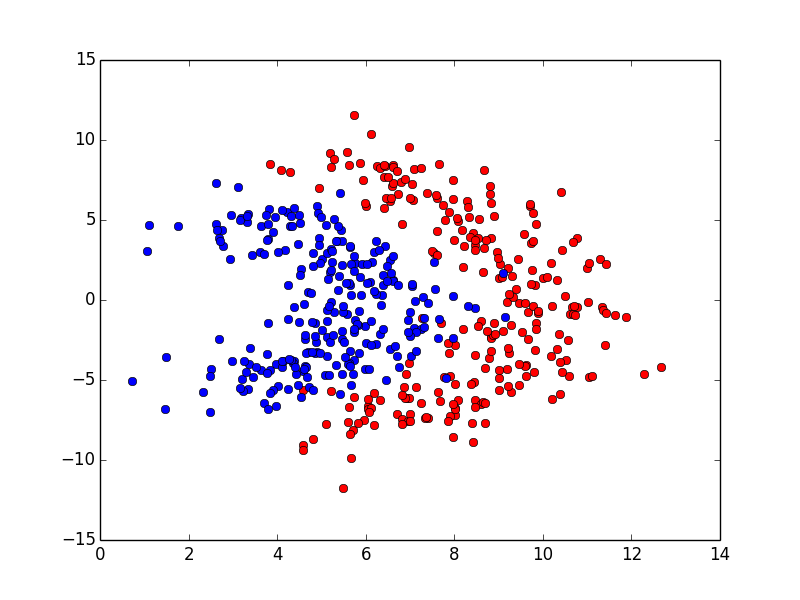
\includegraphics[scale=0.6]{figs/dataset_Lithuanian}
\caption{Lithuanian Data Set}
\label{Figure::lithuanian}
\end{figure}

\begin{figure}[]
\centering
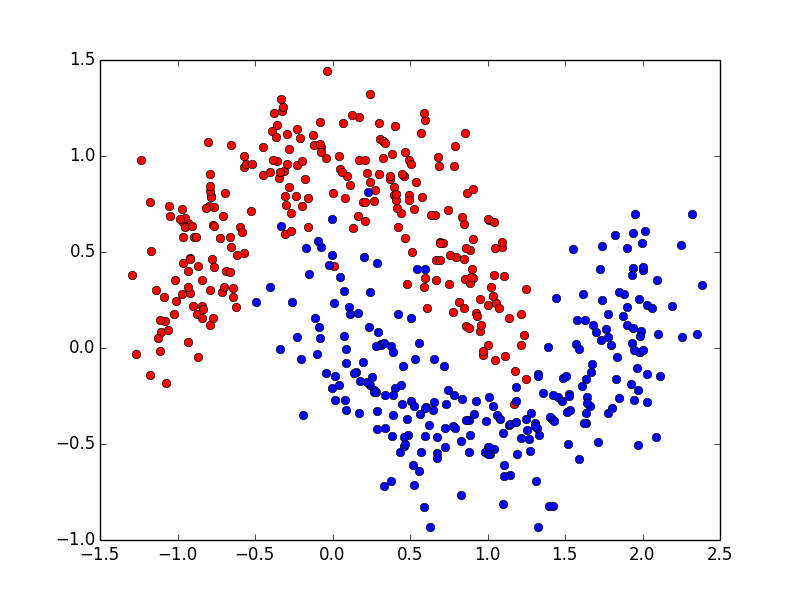
\includegraphics[scale=0.6]{figs/dataset_Banana}
\caption{Banana (Moon) Data Set}
\label{Figure::banana}
\end{figure}

\begin{figure}[]
\centering
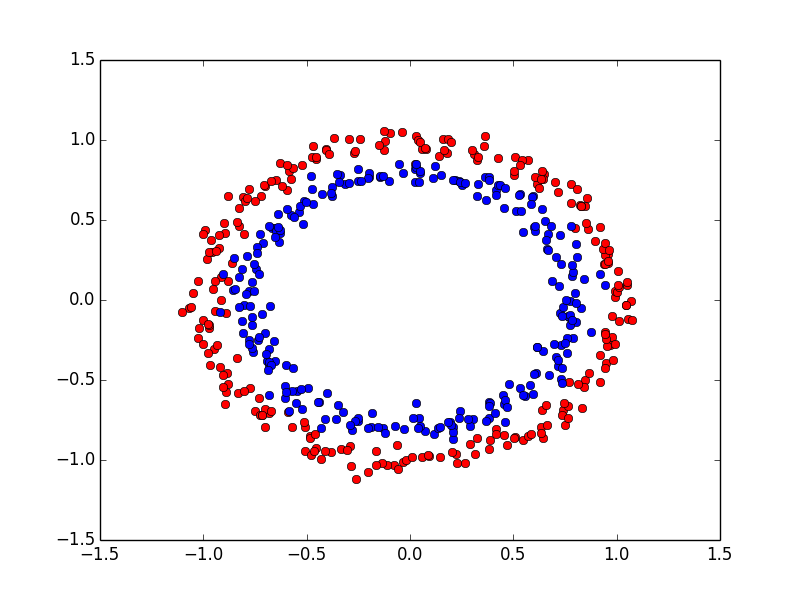
\includegraphics[scale=0.6]{figs/dataset_circle}
\caption{Circle Data Set}
\label{Figure::circle}
\end{figure}

As shown in Figure~\ref{Figure::lithuanian_all}, ~\ref{Figure::banana_all} and ~\ref{Figure::circle_all}, we have different trained detectors on these data sets. None of them, however, can detect all the classes but as we will show later, we can use them to better classify the data set by combining these simple detectors.

\begin{figure}[H]
\centering
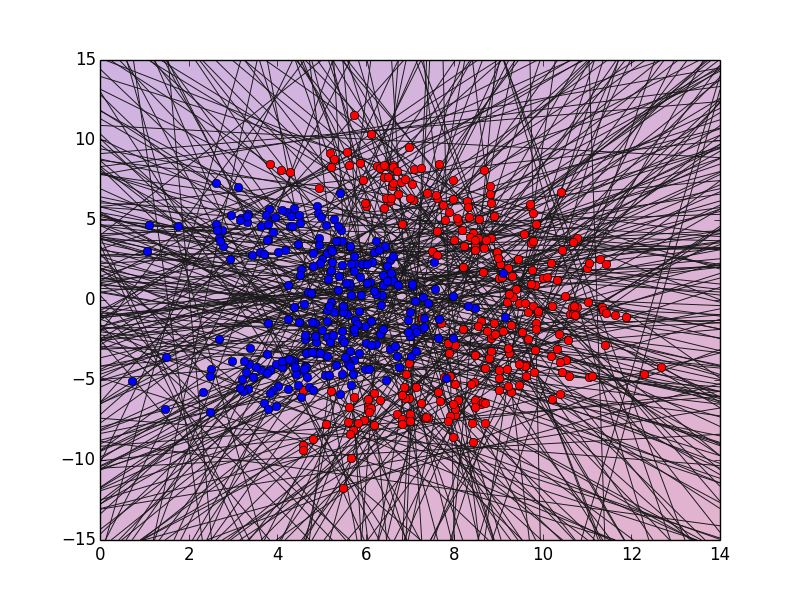
\includegraphics[scale=0.6]{figs/AllClassifiersLithuanian}
\caption{Linear detectors trained on the Lithuanian Data Set}
\label{Figure::lithuanian_all}
\end{figure}

\begin{figure}[H]
\centering
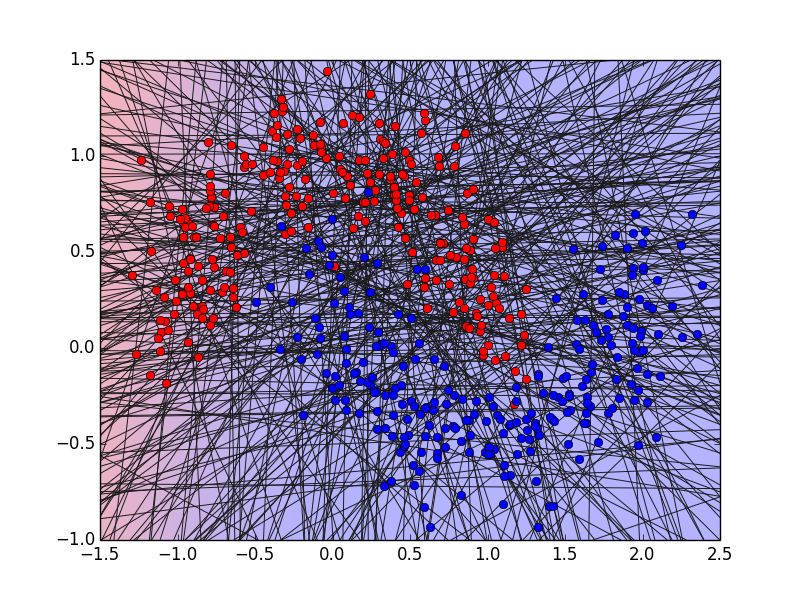
\includegraphics[scale=0.6]{figs/AllClassifiersBanana}
\caption{Linear detectors trained on the Banana (Moon) Data Set}
\label{Figure::banana_all}
\end{figure}

\begin{figure}[H]
\centering
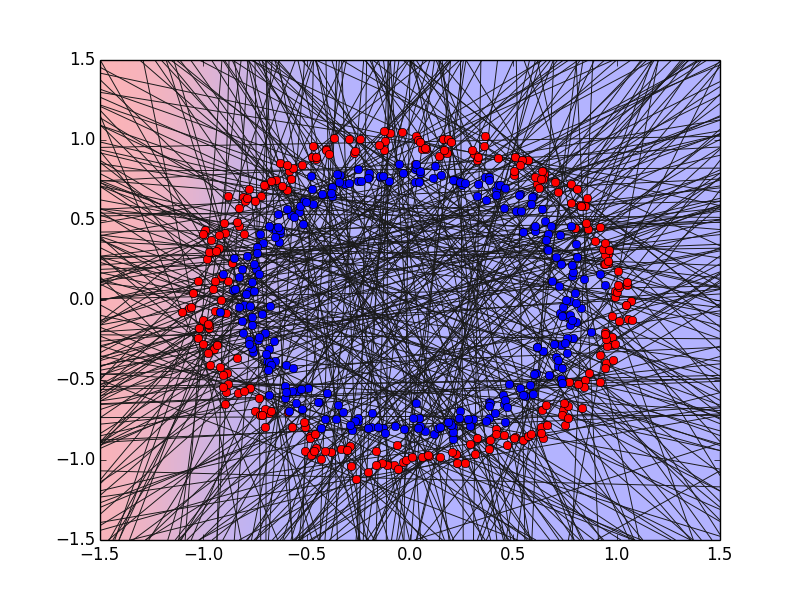
\includegraphics[scale=0.6]{figs/AllClassifiersCircle}
\caption{Linear detectors trained on the Circle Data Set}
\label{Figure::circle_all}
\end{figure}

By selecting the right models and combining them, we can increase the detection rate, as shown in Figures~\ref{fig:ROC_comparison_banana}, ~\ref{fig:ROC_comparison_lithuanian} and ~\ref{fig:ROC_comparison_circle}. The figures on the left show the original detectors and their ROC before the combination. After selecting the proper detectors and combining them together (i.e. after just one iteration), we can reach the accuracy shown on the right figures, which show the combined detectors (in yellow) and their improved ROC curve. The next step is to show why the model generated after the combination provides better results and how we can obtain the same results just by combining parts of trained models.



\begin{figure}[H]
    \centering
    \begin{adjustbox}{minipage=\linewidth,scale=1.1}
    \begin{subfigure}[b]{0.5\columnwidth}
        \centering
        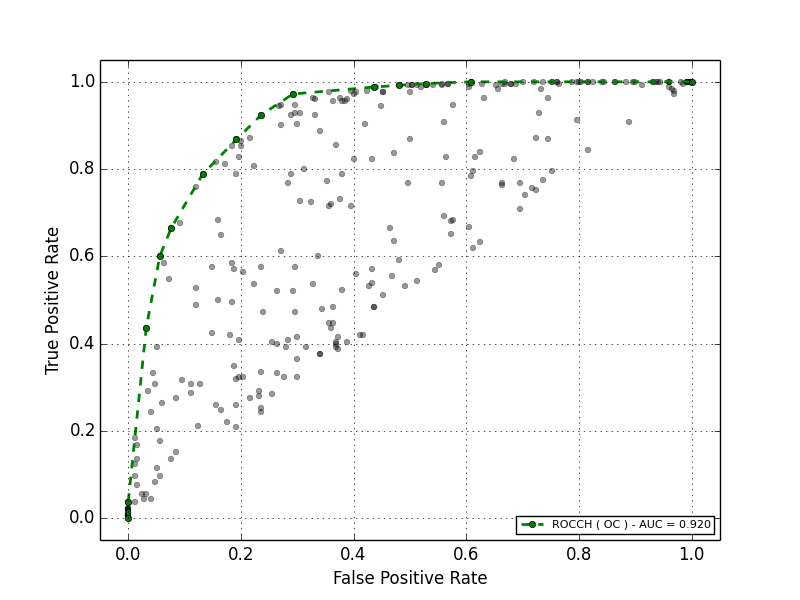
\includegraphics[width=\linewidth]{figs/ROCHLeft-Lithuanian}
        \caption{ROC before combination}
        \label{fig:ROC_left_lithuanian} 
    \end{subfigure}
    \begin{subfigure}[b]{0.5\columnwidth}
        \centering
        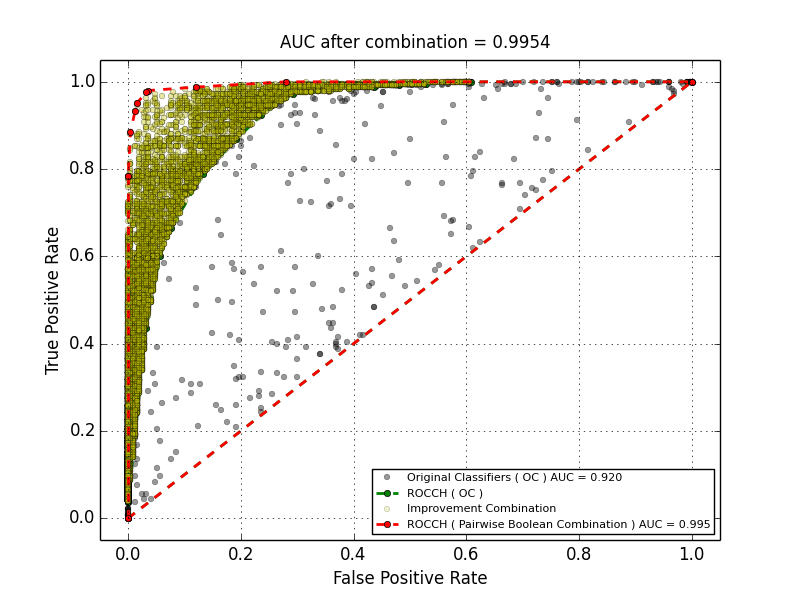
\includegraphics[width=\linewidth]{figs/ROCHRight-Lithuanian}
        \caption{ROC after combination}
        \label{fig:ROC_right_lithuanian}
    \end{subfigure}
    \caption{ROC comparison on Lithuanian data set before and after first round of combination}
    \label{fig:ROC_comparison_lithuanian}
    \end{adjustbox}
\end{figure}


\begin{figure}[H]
    \centering
    \begin{adjustbox}{minipage=\linewidth,scale=1.1}
    \begin{subfigure}[b]{0.5\columnwidth}
        \centering
        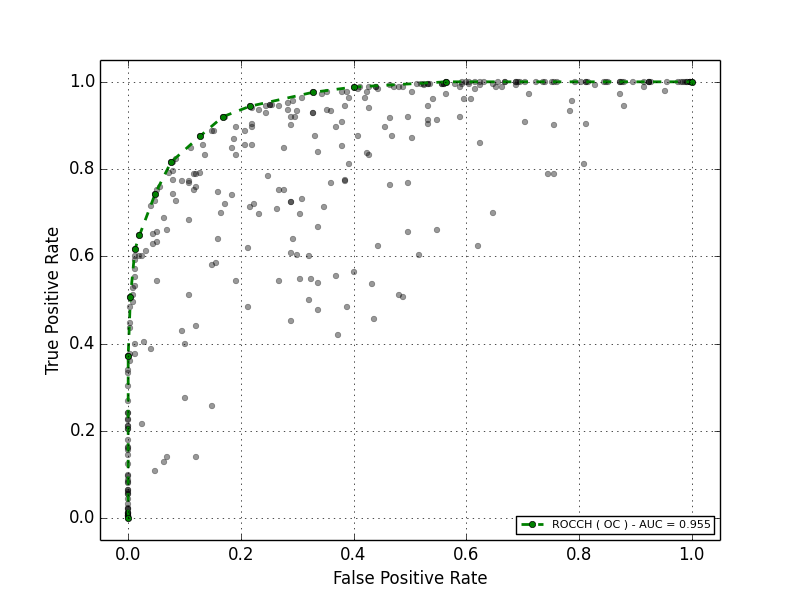
\includegraphics[width=\linewidth]{figs/ROCHLeft-Banana}
        \caption{ROC before combination}
        \label{fig:ROC_left_banana} 
    \end{subfigure}
    \begin{subfigure}[b]{0.5\columnwidth}
        \centering
        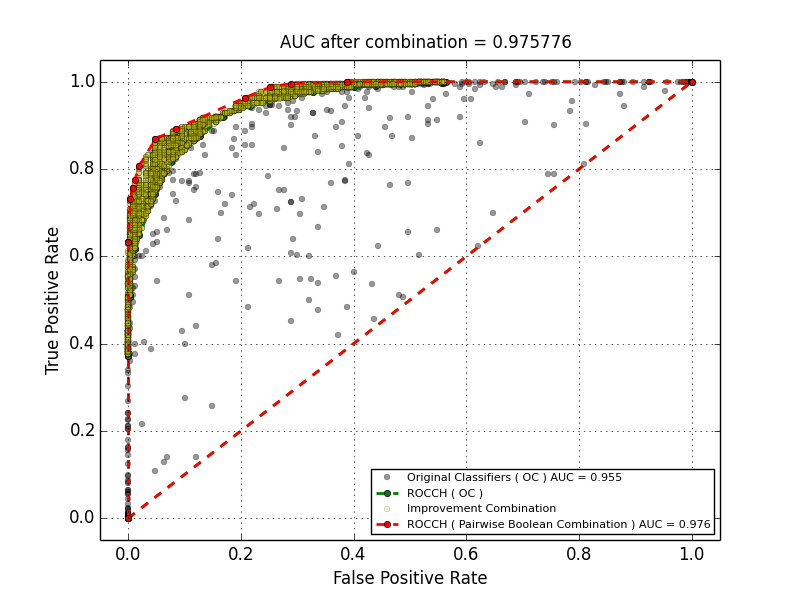
\includegraphics[width=\linewidth]{figs/ROCHRight-Banana}
        \caption{ROC after combination}
        \label{fig:ROC_right_banana}
    \end{subfigure}
    \caption{ROC comparison on Banana data set before and after first round of combination}
    \label{fig:ROC_comparison_banana}
    \end{adjustbox}
\end{figure}

\begin{figure}[H]
    \centering
    \begin{adjustbox}{minipage=\linewidth,scale=1.1}
    \begin{subfigure}[b]{0.5\columnwidth}
        \centering
        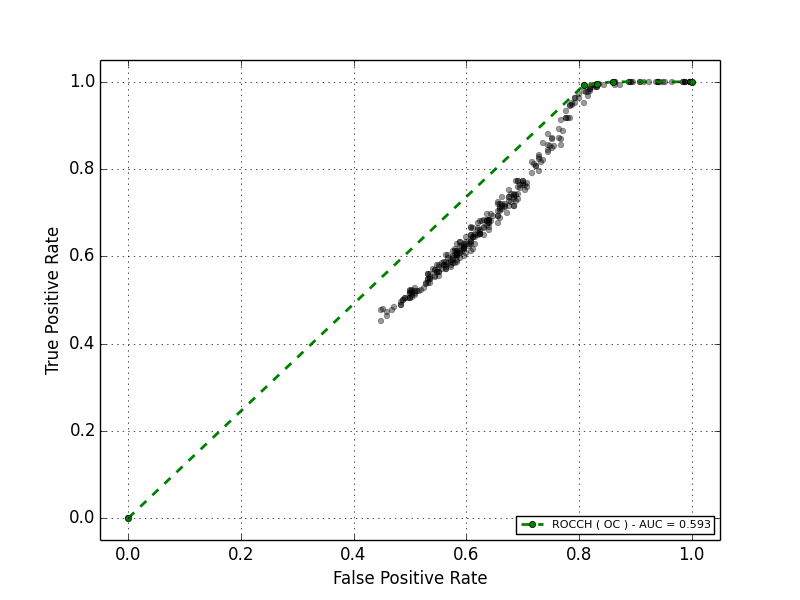
\includegraphics[width=\linewidth]{figs/ROCHLeft-Circle}
        \caption{ROC before combination}
        \label{fig:ROC_left_circle} 
    \end{subfigure}
    \begin{subfigure}[b]{0.5\columnwidth}
        \centering
        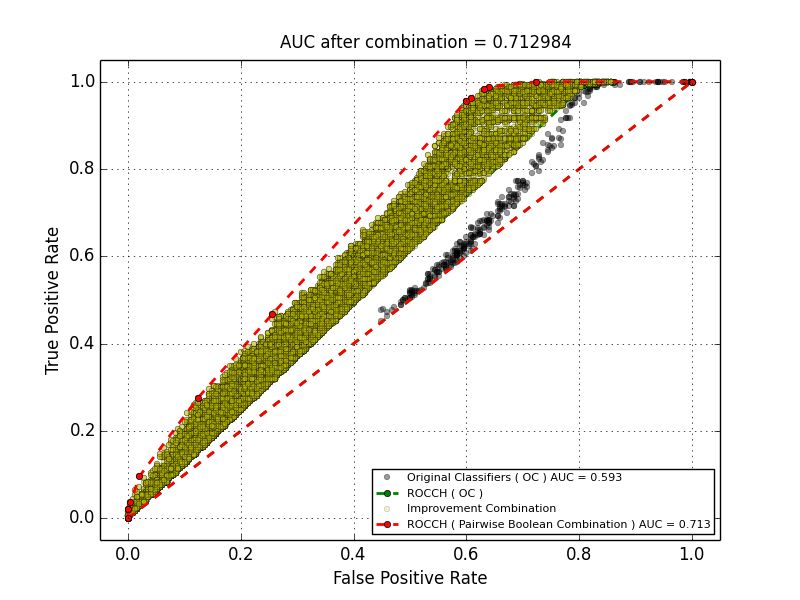
\includegraphics[width=\linewidth]{figs/ROCHRight-Circle}
        \caption{ROC after combination}
        \label{fig:ROC_right_circle}
    \end{subfigure}
    \caption{ROC comparison on Circle data set before and after first round of combination}
    \label{fig:ROC_comparison_circle}
    \end{adjustbox}
\end{figure}

For each data set, we show that there is no single detector that can classify the data set properly. 

\begin{figure}[t!] % "[t!]" placement specifier just for this example
\begin{subfigure}{0.48\textwidth}
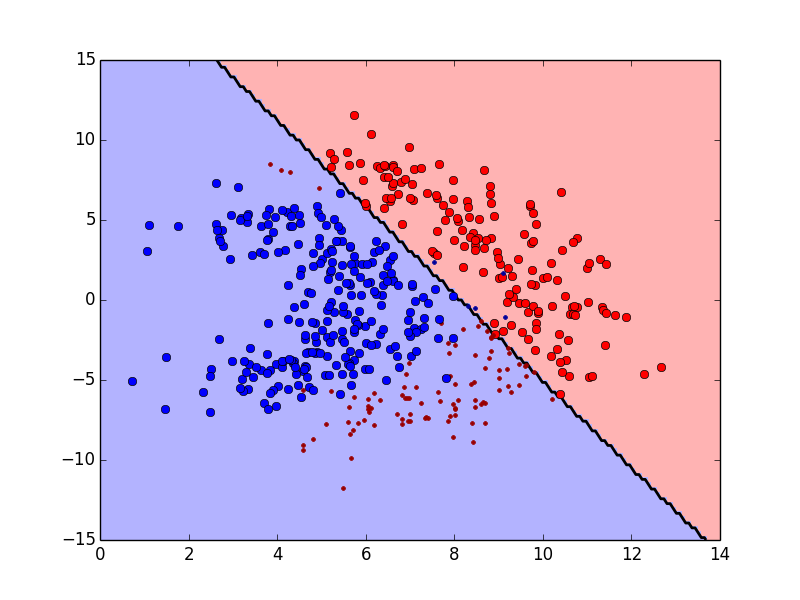
\includegraphics[width=\linewidth]{figs/Lithuanian/20All-Classifiers}
\caption{First subfigure} \label{fig:Lithuanian_all_single_a}
\end{subfigure}\hspace*{\fill}
\begin{subfigure}{0.48\textwidth}
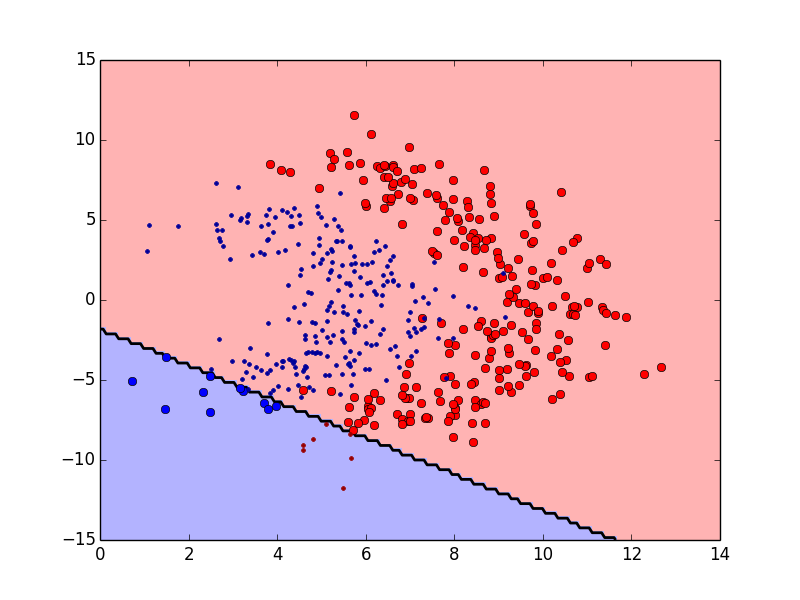
\includegraphics[width=\linewidth]{figs/Lithuanian/43All-Classifiers}
\caption{Second subfigure} \label{fig:Lithuanian_all_single_b}
\end{subfigure}

\medskip
\begin{subfigure}{0.48\textwidth}
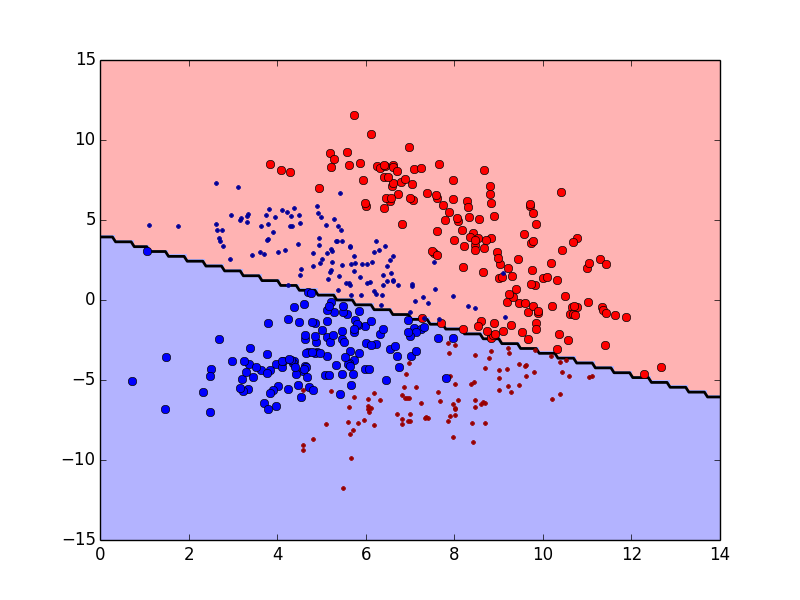
\includegraphics[width=\linewidth]{figs/Lithuanian/44All-Classifiers}
\caption{Third subfigure} \label{fig:Lithuanian_all_single_c}
\end{subfigure}\hspace*{\fill}
\begin{subfigure}{0.48\textwidth}
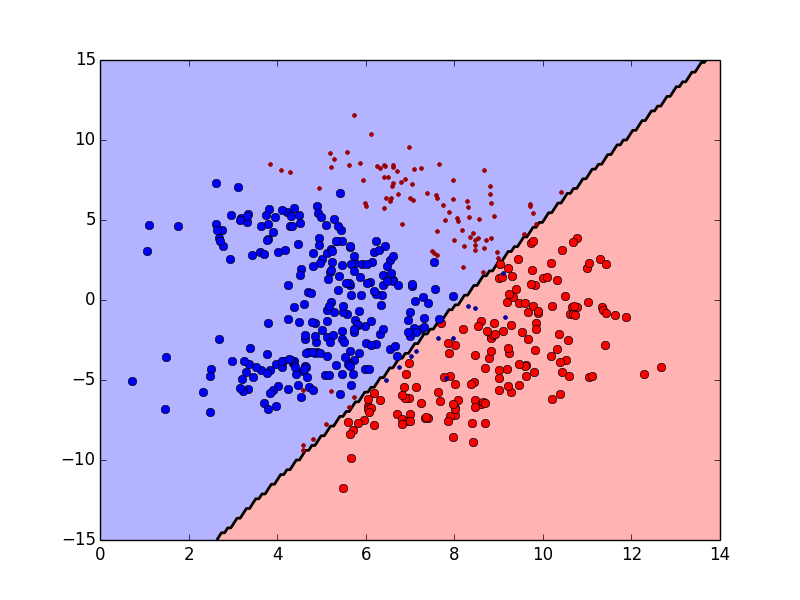
\includegraphics[width=\linewidth]{figs/Lithuanian/65All-Classifiers}
\caption{Fourth subfigure} \label{fig:Lithuanian_all_single_d}
\end{subfigure}

\medskip
\begin{subfigure}{0.48\textwidth}
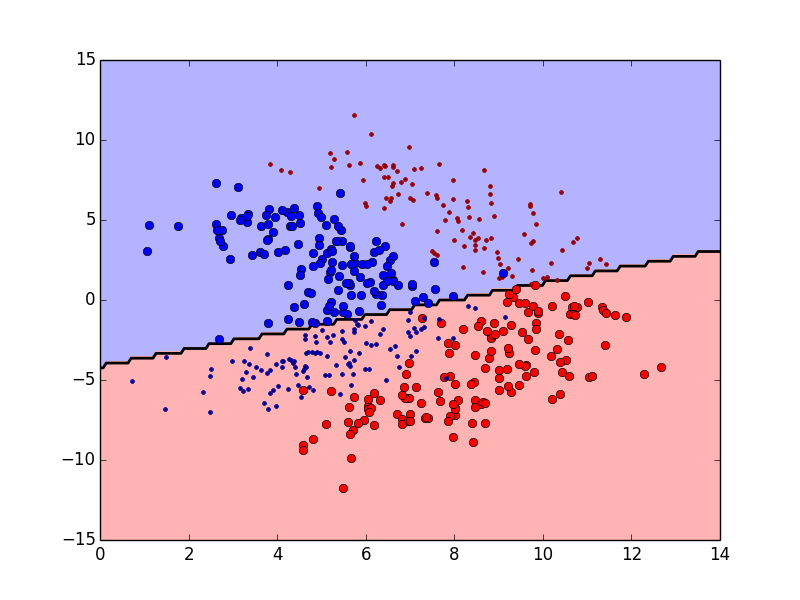
\includegraphics[width=\linewidth]{figs/Lithuanian/118All-Classifiers}
\caption{Fifth subfigure} \label{fig:Lithuanian_all_single_e}
\end{subfigure}\hspace*{\fill}
\begin{subfigure}{0.48\textwidth}
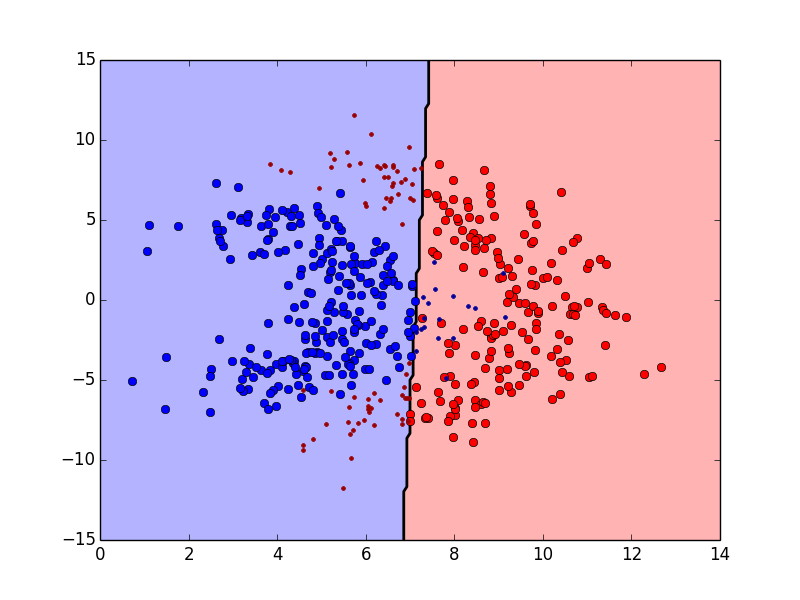
\includegraphics[width=\linewidth]{figs/Lithuanian/146All-Classifiers}
\caption{Sixth subfigure} \label{fig:Lithuanian_all_single_f}
\end{subfigure}

\caption{Some of best LDA ( Linear Discriminant Analysis) that can be trained on Lithuanian data set} \label{fig:Lithuanian_all_single}
\end{figure}

As it is shown in Figure~\ref{fig:Lithuanian_all_single}, with just one LDA, we cannot classify all the classes 100\%. We can, however, see that it is possible to choose two of these detectors and combine them to obtain a better result. As it is shown in Figure~\ref{fig:Dataset_ROC_Lithuanian}, we select detector from Figure~\ref{fig:Lithuanian_all_single_a}  and detectors from ~\ref{fig:Lithuanian_all_single_d} and combine them together.

\begin{figure}[H]
    \centering
    \begin{adjustbox}{minipage=\linewidth,scale=1.1}
    \begin{subfigure}[b]{0.5\columnwidth}
        \centering
        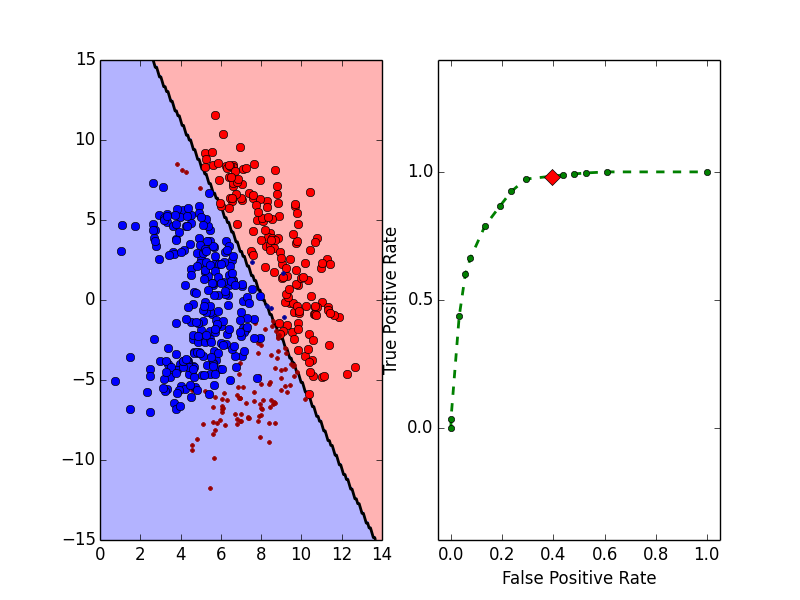
\includegraphics[width=\linewidth]{figs/Lithuanian/20Dataset-ROC}
        \caption{First selected LDA}
        \label{fig:Dataset_ROC_Lithuanian_a} 
    \end{subfigure}
    \begin{subfigure}[b]{0.5\columnwidth}
        \centering
        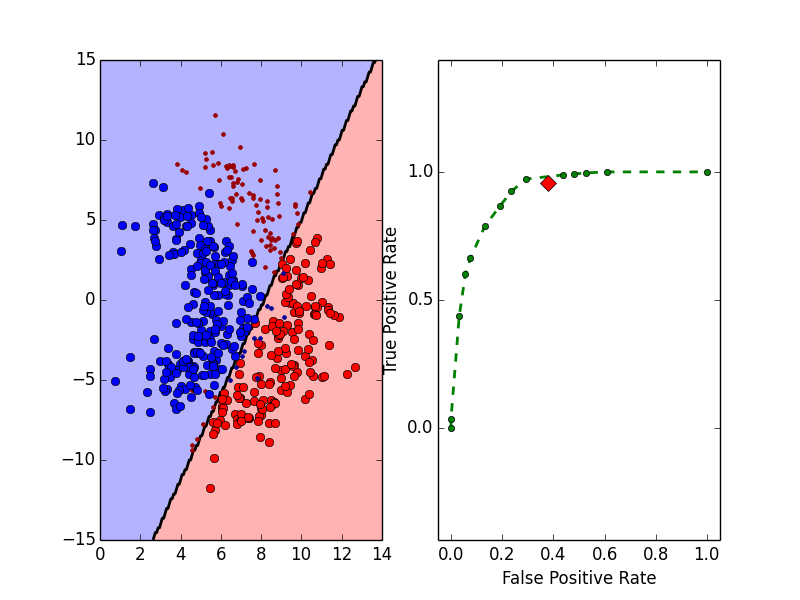
\includegraphics[width=\linewidth]{figs/Lithuanian/65Dataset-ROC}
        \caption{Second selected LDA}
        \label{fig:Dataset_ROC_Lithuanian_b}
    \end{subfigure}
    \caption{Selected LDA and their respective point compare to current ROC}
    \label{fig:Dataset_ROC_Lithuanian}
    \end{adjustbox}
\end{figure}

If we combine these two detectors with an $AND$ operation,  as shown in Figure~\ref{fig::combined_lithuanian_roc},  we can obtain a better result. The  red point is the mapping of the combined detectors. As we can see if we recalculate the ROC based on this new generated point we will have a greater AUC.

\begin{figure}[H]
\centering
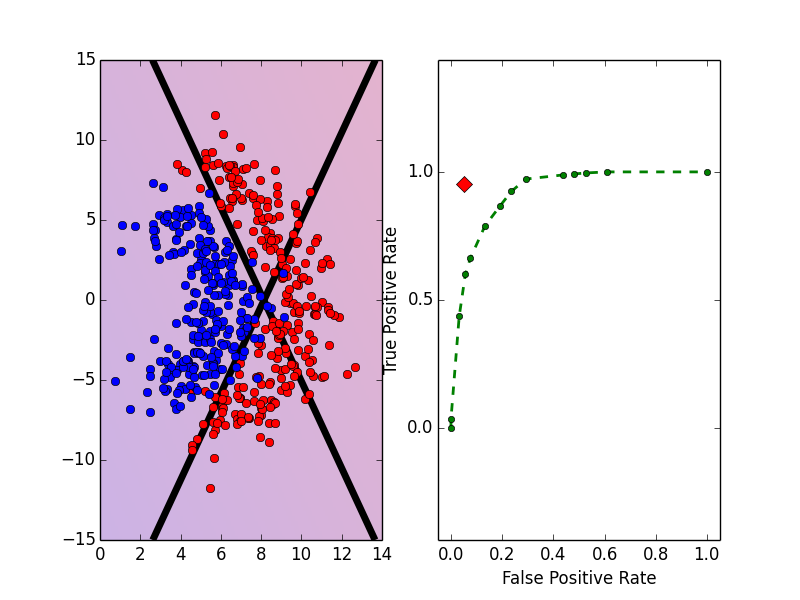
\includegraphics[scale=0.6]{figs/Lithuanian/9999999-combined_All-Classifiers}
\caption{Selected detectors and respective combined point on ROC curve}
\label{fig::combined_lithuanian_roc}
\end{figure}


A similar approach can be applied to the Banana data set. As you can see in Figure~\ref{fig:Banana_all_single}, like for the Lithuania data set, it is not possible to classify the data set completely with one detector.  In this specific example, we need at least three detectors in order to classify the data in an accurate way. 

\begin{figure}[t!] % "[t!]" placement specifier just for this example
\begin{subfigure}{0.48\textwidth}
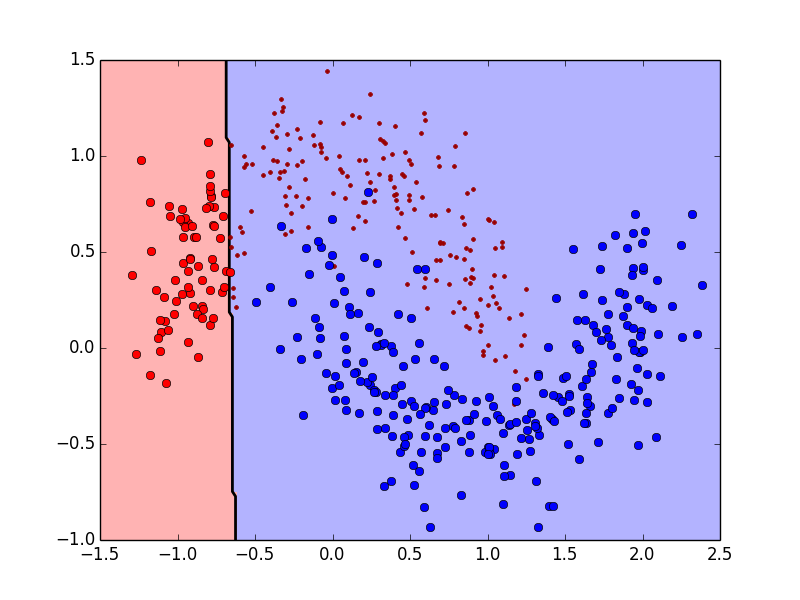
\includegraphics[width=\linewidth]{figs/Banana/2All-Classifiers}
\caption{First subfigure} \label{fig:Banana_all_single_a}
\end{subfigure}\hspace*{\fill}
\begin{subfigure}{0.48\textwidth}
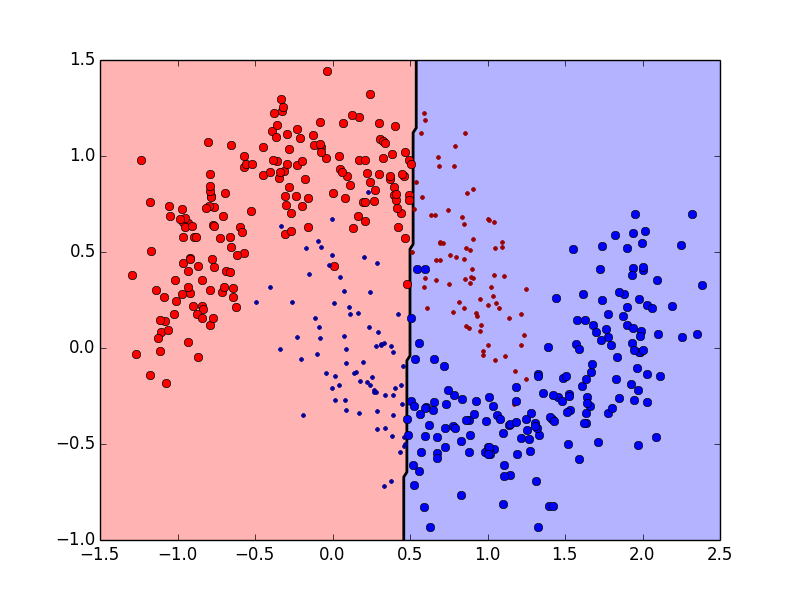
\includegraphics[width=\linewidth]{figs/Banana/12All-Classifiers}
\caption{Second subfigure} \label{fig:Banana_all_single_b}
\end{subfigure}

\medskip
\begin{subfigure}{0.48\textwidth}
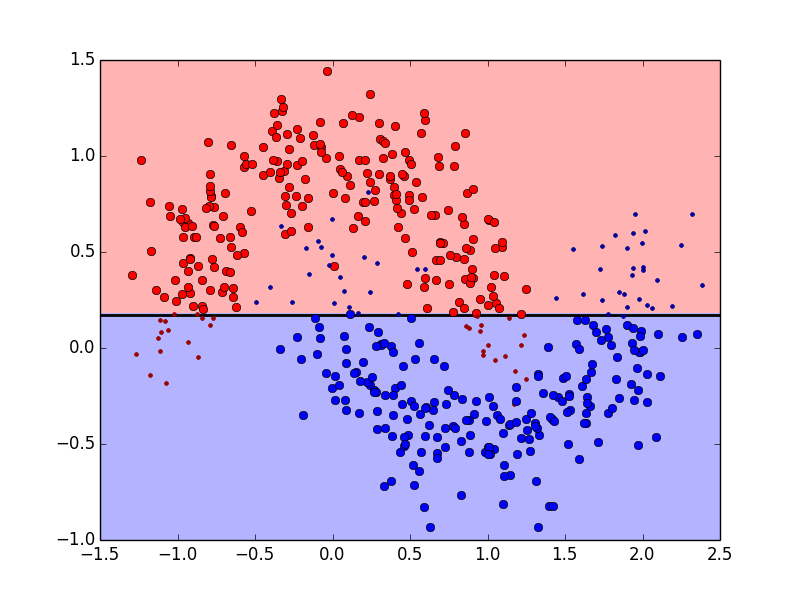
\includegraphics[width=\linewidth]{figs/Banana/22All-Classifiers}
\caption{Third subfigure} \label{fig:Banana_all_single_c}
\end{subfigure}\hspace*{\fill}
\begin{subfigure}{0.48\textwidth}
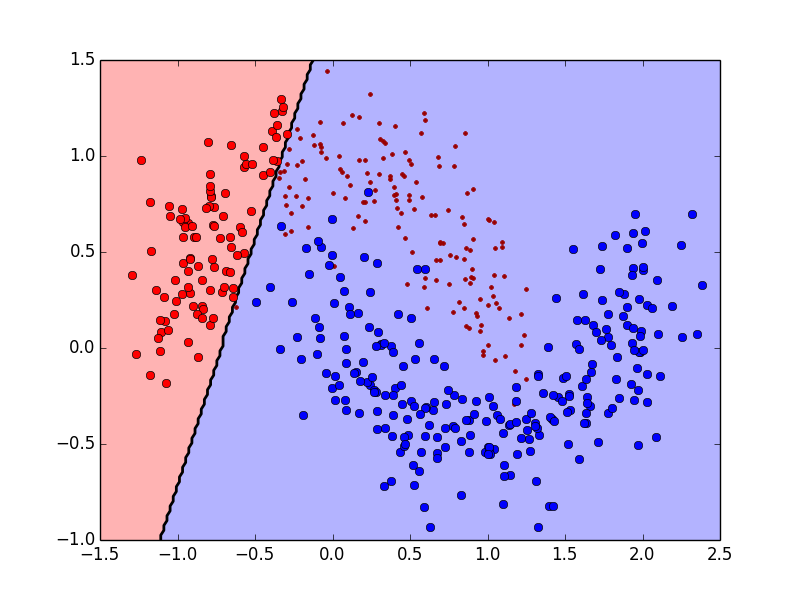
\includegraphics[width=\linewidth]{figs/Banana/54All-Classifiers}
\caption{Fourth subfigure} \label{fig:Banana_all_single_d}
\end{subfigure}

\medskip
\begin{subfigure}{0.48\textwidth}
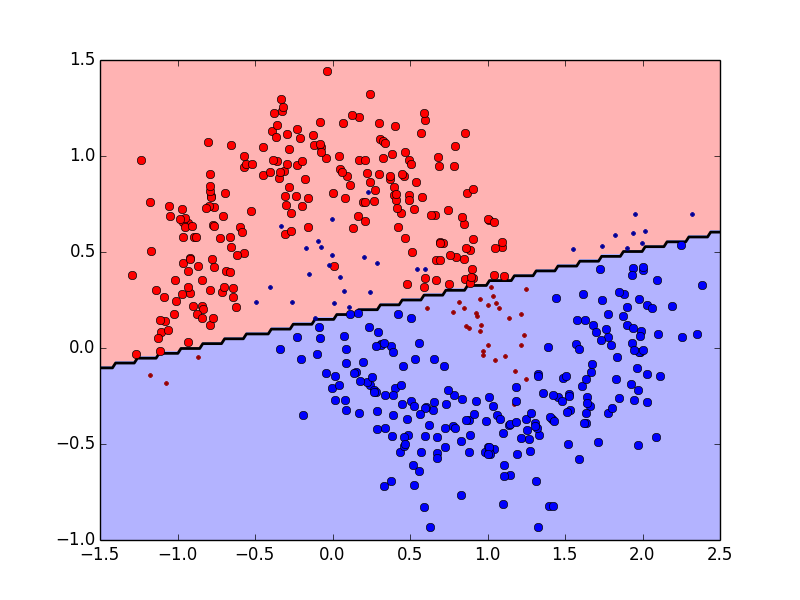
\includegraphics[width=\linewidth]{figs/Banana/147All-Classifiers}
\caption{Fifth subfigure} \label{fig:Banana_all_single_e}
\end{subfigure}\hspace*{\fill}
\begin{subfigure}{0.48\textwidth}
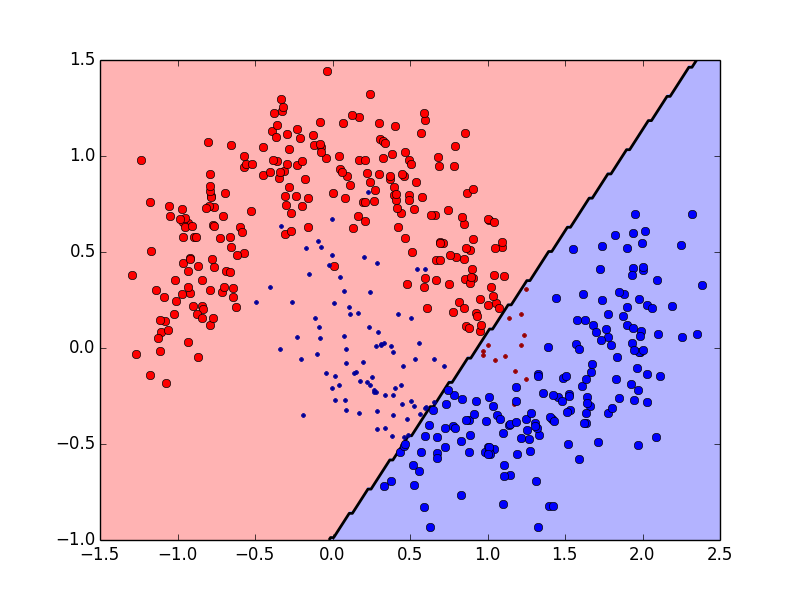
\includegraphics[width=\linewidth]{figs/Banana/160All-Classifiers}
\caption{Sixth subfigure} \label{fig:Banana_all_single_f}
\end{subfigure}

\caption{Some of best LDA ( Linear Discriminant Analysis) that can be trained on Banana data set} \label{fig:Banana_all_single}
\end{figure}

Based on the observation in this example it is better to select 3 detectors in order to be classify the data set, if we select detector in Figure~\ref{fig:Banana_all_single_a}, Figure~\ref{fig:Banana_all_single_c} and Figure~\ref{fig:Banana_all_single_f}  and combine them together we should expect to get the most accurate result among all other detectors. in Figure~\ref{fig::combined_banana_roc} you can see all these detectors in one plot.


\begin{figure}[H]
\centering
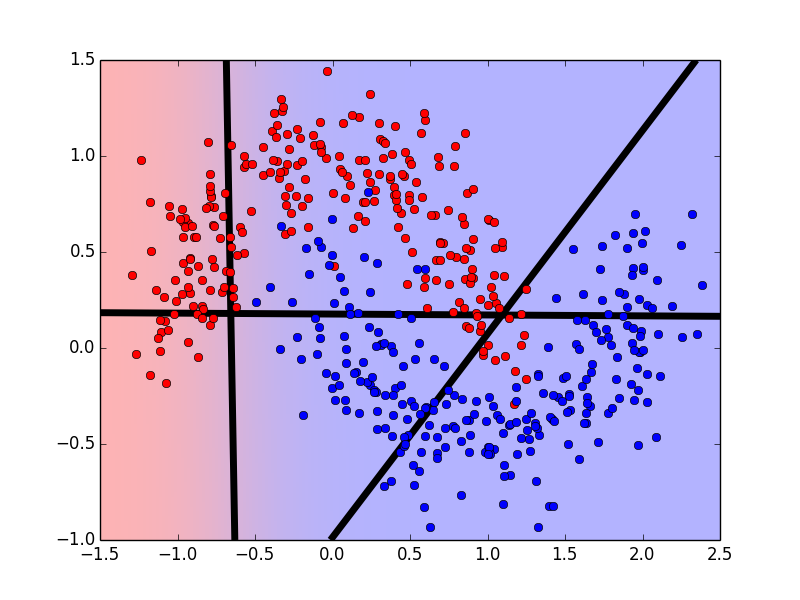
\includegraphics[scale=0.6]{figs/Banana/9999999-combined_selected_before_combination}
\caption{Best potential selected detectors on Banana data set}
\label{fig::combined_banana_roc}
\end{figure}

These examples show that it is not always necessary to train complex models, which takes time and resources, over the data set to obtain the best result possible. The same result can be achieved by combining two or more simple models, which can be trained much faster. Also by increasing the number these simple models, we can cover most of the cases (including the outliers) in the data set. Besides, even if we decide to train complex models, there is no guarantee that we can obtain the best results since every model has its own weaknesses. This said, some sort of combination is needed to help improve the result. In the next chapter we show how we can select a set of meaningful models that can help improve the result since it is not possible to train thousands of models and combine them all together. 

The Circle data set is a good example where doing combination in an iterative way improves the accuracy, as shown in Figure~\ref{fig:Circle_all_single}. We could not find any two detectors that can be combined  to classify the whole data set. What we need here is to select all of these detectors and start  combining them two by two iteratively. In Figure~\ref{fig::combined_circle_roc}, we show the result of classifying iteratively  the whole data set with the help of a few simple detectors.


\begin{figure}[H] % "[t!]" placement specifier just for this example
\begin{subfigure}{0.48\textwidth}
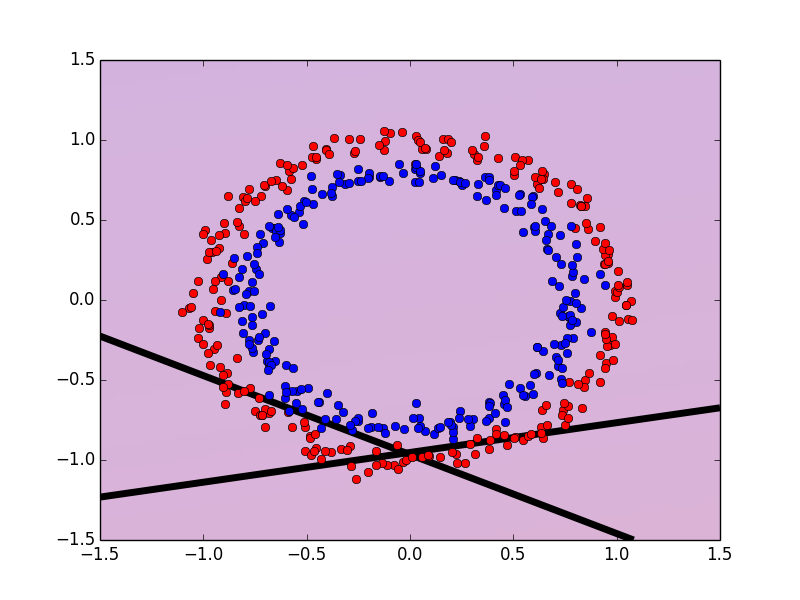
\includegraphics[width=\linewidth]{figs/Circle/11-two-circle}
\caption{First subfigure} \label{fig:Circle_all_single_a}
\end{subfigure}\hspace*{\fill}
\begin{subfigure}{0.48\textwidth}
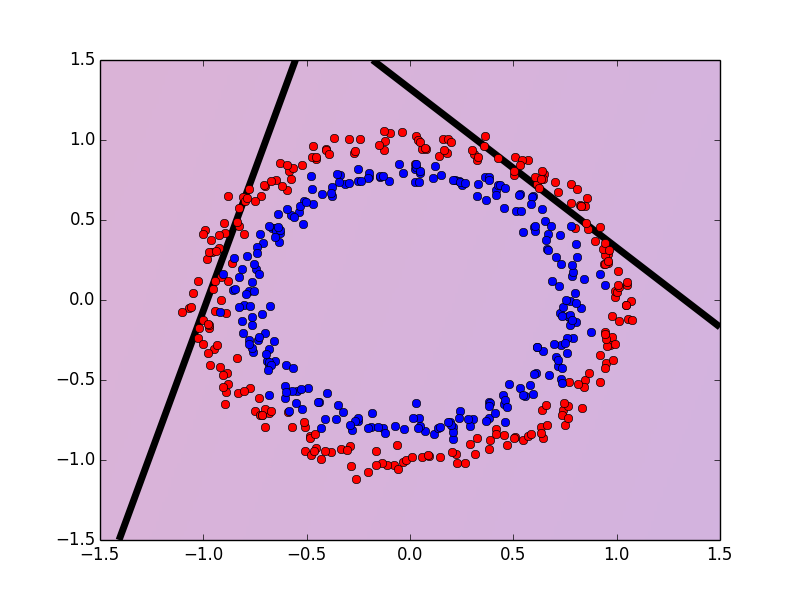
\includegraphics[width=\linewidth]{figs/Circle/22-two-circle}
\caption{Second subfigure} \label{fig:Circle_all_single_b}
\end{subfigure}

\medskip
\begin{subfigure}{0.48\textwidth}
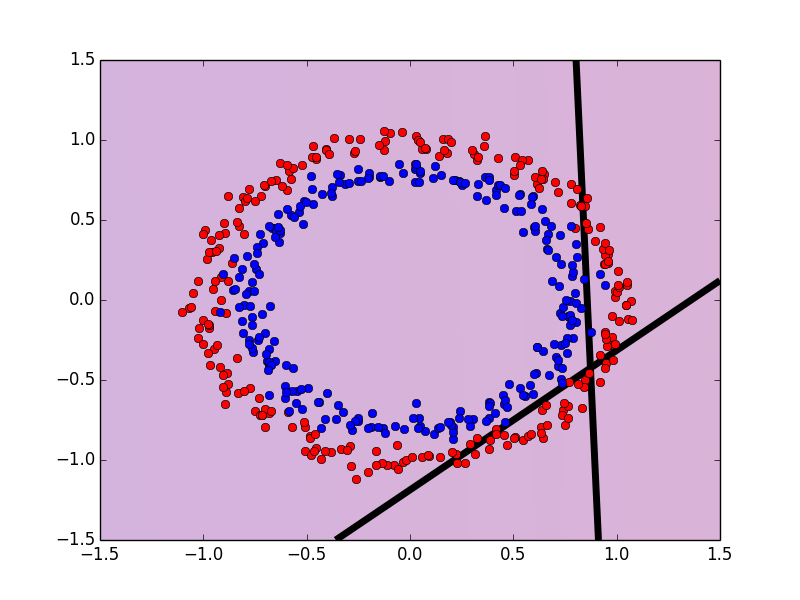
\includegraphics[width=\linewidth]{figs/Circle/33-two-circle}
\caption{Third subfigure} \label{fig:Circle_all_single_c}
\end{subfigure}\hspace*{\fill}
\begin{subfigure}{0.48\textwidth}
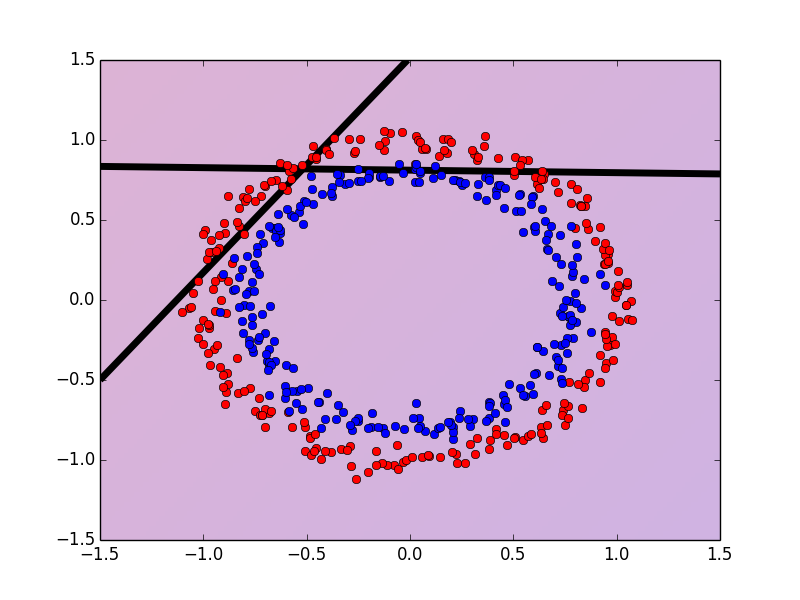
\includegraphics[width=\linewidth]{figs/Circle/44-two-circle}
\caption{Fourth subfigure} \label{fig:Circle_all_single_d}
\end{subfigure}

\medskip
\begin{subfigure}{0.48\textwidth}
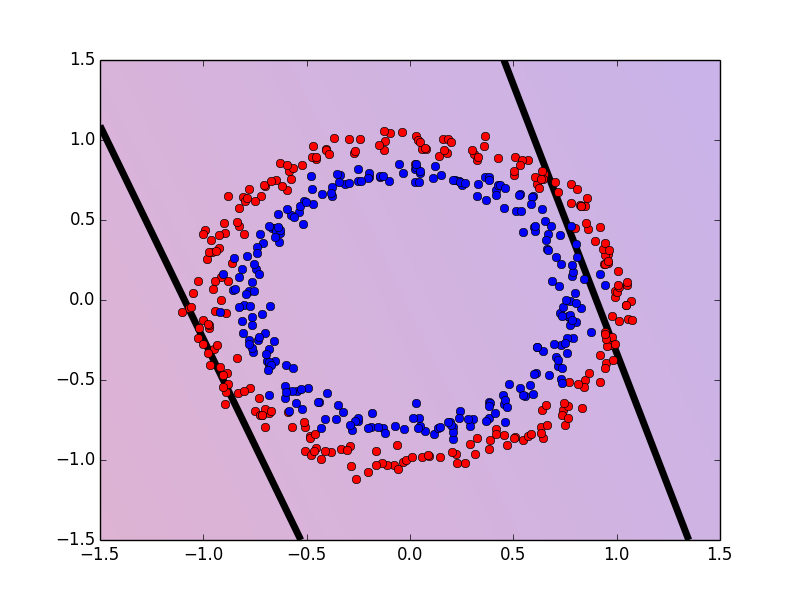
\includegraphics[width=\linewidth]{figs/Circle/55-two-circle}
\caption{Fifth subfigure} \label{fig:Circle_all_single_e}
\end{subfigure}\hspace*{\fill}
\begin{subfigure}{0.48\textwidth}
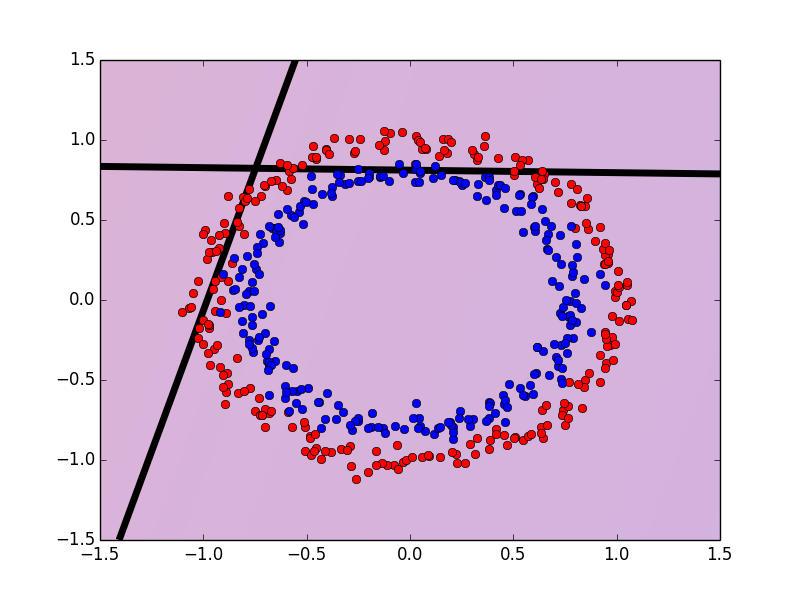
\includegraphics[width=\linewidth]{figs/Circle/66-two-circle}
\caption{Sixth subfigure} \label{fig:Circle_all_single_f}
\end{subfigure}

\caption{Series of 2 selected LDA ( Linear Discriminant Analysis) that can be trained and combined on the Circle data set} \label{fig:Circle_all_single}
\end{figure}

\begin{figure}[H]
\centering
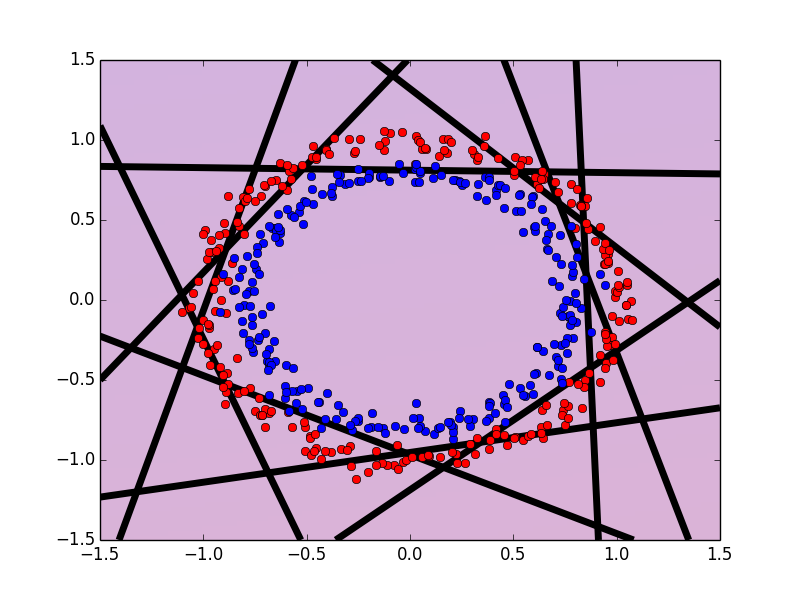
\includegraphics[scale=0.6]{figs/Circle/9999999-combined_selected_before_combination}
\caption{Best potential selected detectors on the Circle data set}
\label{fig::combined_circle_roc}
\end{figure}





\chapter{Pruning} \label{chapter3}


 \section{Introduction}
\label{sec:chap3-introduction}

Pruning is a very popular practice for decreasing the cost and time of combining multiple detectors. There are two main challenges when it comes to pruning. The first one is to determine where pruning should be applied (e.g., feature level, model level, etc.) and the second challenge is to determine the pruning criteria.

Generally speaking, pruning can be done at four different levels: sensor level, feature level, matching score level, and decision level \cite{Tao2009}, as illustrated in Figure~\ref{fig::level_of_pruning}

 In this thesis, the main focus of pruning detectors is at the decision level. However, there are some scenarios that requires pruning at the matching score level. For example, when there are thousands of detectors; it is not beneficial to convert them into a few response vectors and combine everything together. The reason is that we will have too many redundant response vectors, which hinders the efficiency of the pruning process.


\begin{figure}[]
\centering
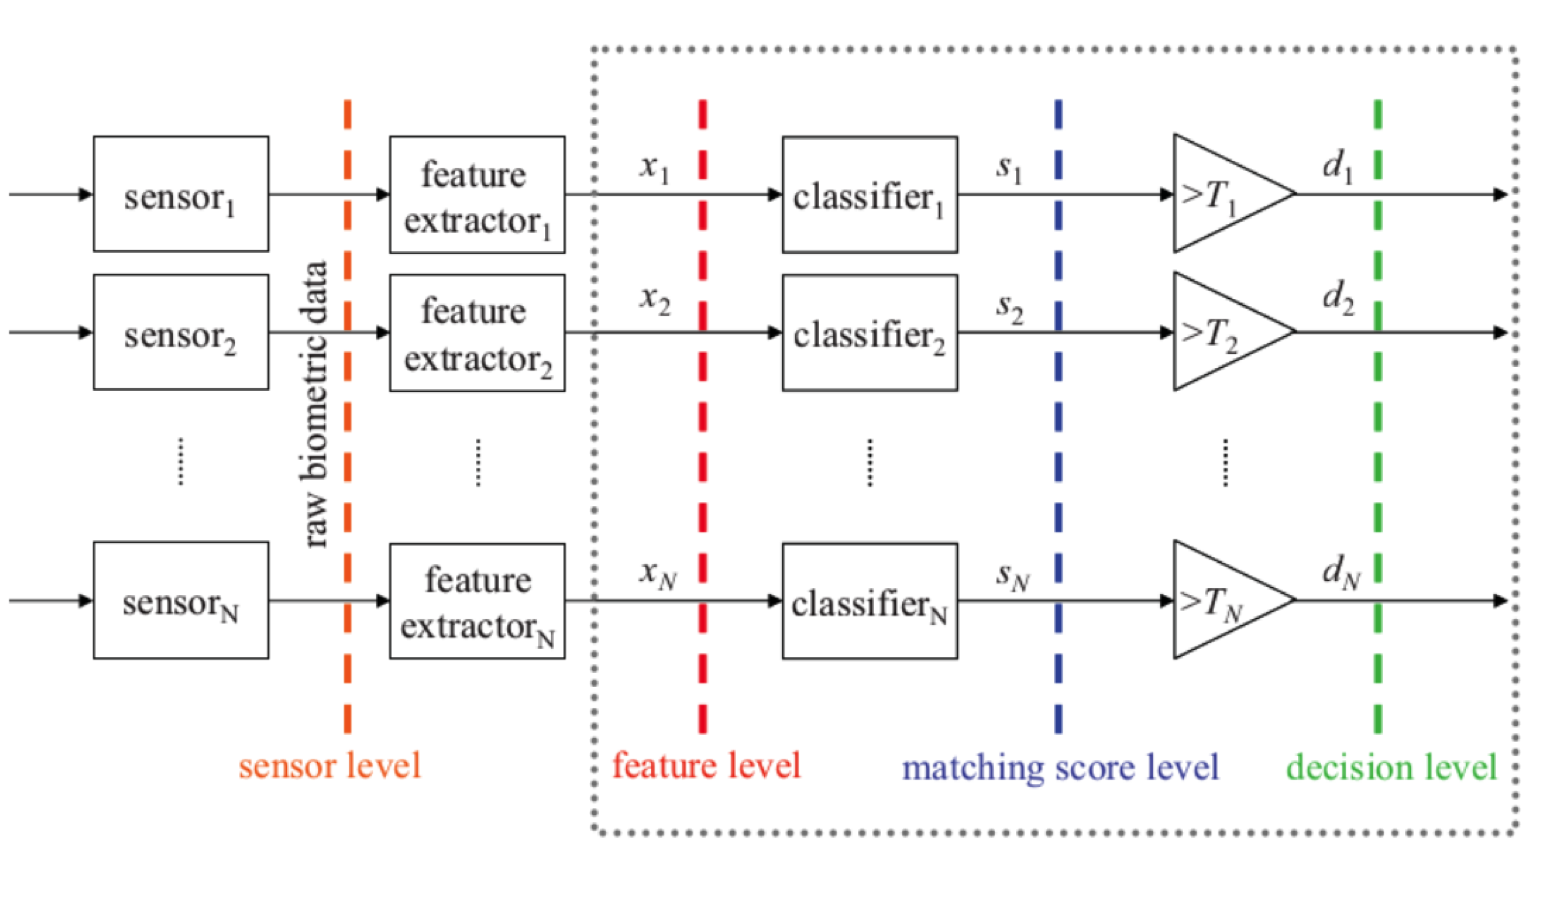
\includegraphics[width=1\linewidth]{figs/level-of-pruning}
\caption{Different levels of combination or pruning: sensor level, feature level, matching score level, and decision level \cite{Tao2009}.}
\label{fig::level_of_pruning}
\end{figure}

After seeing different levels where pruning can be applied, the question is how to prune the pool of available detectors and make a basket of reasonable detectors. To have a reasonable basket of remaining detectors, two criteria should be considered.  

Firstly, we have to define some accurate detectors in the basket, with this we guarantee that the minimum accuracy we obtain after pruning and the combination is not worse than any of the detectors we had in the pool. Also, by choosing and combining the accurate ones, we increase the probability of getting better results than combining two random or naïve detectors.  

The second criteria is the diversity in the basket of detectors. If very similar detectors  are selected  in the basket, we should not expect to see a major improvement after combining. One way to increase the diversity of the basket is to try to find and select detectors that complement the errors of already selected detectors. Since we have already selected accurate detectors in the basket, it is a good practice to choose the detectors that complement the errors these detectors exhibit. 

To see the importance of diversity and how it can help to improve the result of the combination, we show in the following example, the importance of selecting the initial detectors and respective detectors compare to them especially, the ones that tries to complement first detector's errors. By combining these two detectors with a right Boolean operator we will reach a very promising result. As it is shown in Figure~\ref{fig::accurate_detector}, among all the trained detectors, we only need to find a way to select one detector that is accurate,and in Figure~\ref{fig::diverse_detector}, we demonstrate how to select a detector, that is very diverse to previously selected ones in order to increase the chance of getting better results after combining. The two selected detectors in Figure~\ref{fig::accurate_detector} and Figure~\ref{fig::diverse_detector} are completing each other errors.


\begin{figure}[H]
\centering
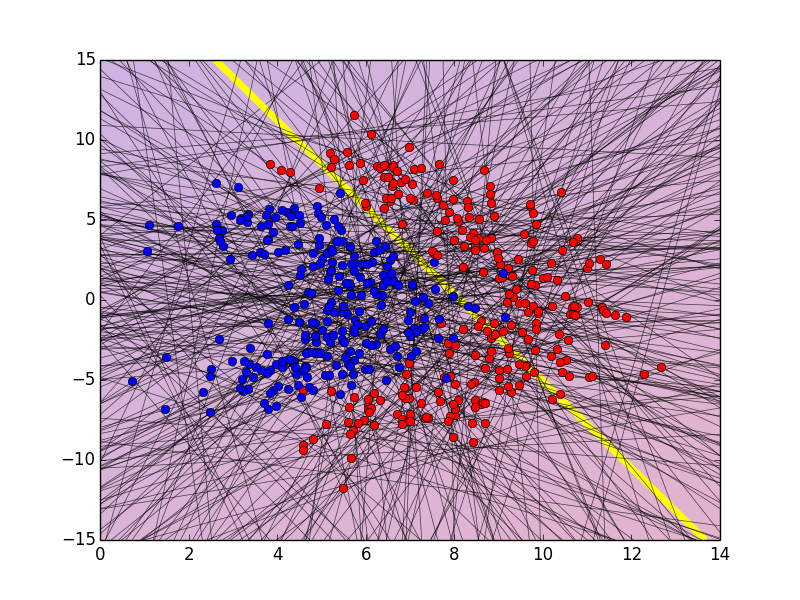
\includegraphics[width=1\linewidth]{figs/Lithuanian/Initial_detectors}
\caption{Selecting accurate detectors}
\label{fig::accurate_detector}
\end{figure}

\begin{figure}[H]
\centering
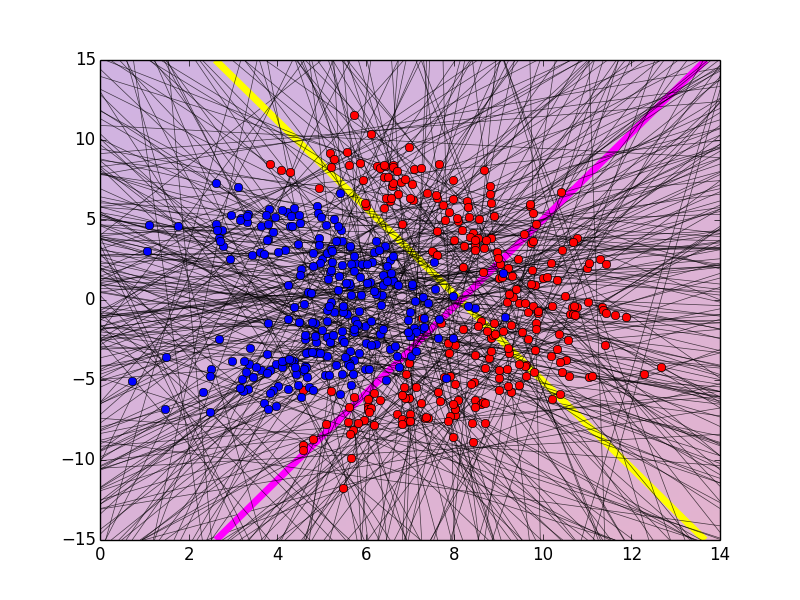
\includegraphics[width=1\linewidth]{figs/Lithuanian/complement_detectors}
\caption{Selecting diverse detector compares to previously selected}
\label{fig::diverse_detector}
\end{figure}


\section{Pruning Boolean Combination (PBC) Approach}
\label{sec:pbc}

In this section, we describe our Pruned Boolean Combination (PBC) algorithm, which is based on two novel pruning techniques that select a subset of diverse and accurate detectors for combination, while discarding the remaining ones, this happened at decision level.
PBC can avoid both the exponential explosion of combinations provided by the brute-force approach and the sequential combination of IBC.
The main difference is that the PBC algorithm proceeds by thresholding all available soft detectors into crisp ones.
This step is, in fact, not essential for PBC because thresholding could be done outside the algorithm and the crisp detectors are directly input for pruning.
In contrast with IBC, all available crisp detectors are input to one of the proposed pruning techniques, MinMax-Kappa or ROCCH-Kappa described in Section~\ref{sub:minmax-kappa}~and~\ref{sub:rocch-kappa}, to select the best subset of crisp detectors for Boolean combination and control its size $U$ (i.e., the number of combined detectors).
Without pruning brute-force pairwise combination of all available detectors may not be feasible for large number of detectors, $\mathcal{O}({N^2})$ (where N is number of available detectors), for further details see Section~\ref{sub:complexity}.
 
After seeing the main pruning idea in Section~\ref{sub:minmax-kappa}~and~\ref{sub:rocch-kappa} we introduce a different distance correlation (measure of agreement between vecotrs or dependence coefficient) ~\ref{sec:dcov-} rather than kappa to show that the results of PBC are consistent, and as long as a proper measure is used we can get promising result either using it with MinMax- or ROCCH-. In Section~\ref{sub:minmax-rocch-dcov} we explained how we used the MinMax and ROCCH technique again and just changed the measure of agreement from kappa to dCor or dCov to prune the pool of detectors.

The boost in performance achieved with an ensemble of detectors is often attributed to the concept of diversity.
While it is generally accepted that an ensemble should contain diverse models to improve the performance, there is no clear definition of diversity neither a consensus about the measure of diversity and its computation.
In practice, several measures of diversity have been proposed to quantify the level of agreement or measure the dependency among the ensemble members \cite{Kuncheva2003b}.


%%%%%%%%%%%%%%%%%%%%%%%%%%%%%%%%%%
\subsection{Kappa Measure}
\label{sec:kappa}

Cohen's Kappa statistic (or simply Kappa hereafter) is one of the well-known and widely used measure of agreement between raters \cite{Cohen1995a}.
Kappa has lately gained some popularity for ensemble combination, especially the Kappa-error diagrams which help visualizing individual accuracy and diversity in a two dimensional plot \cite{Margineantu1997,Kunchev2013}.
Our pruning techniques, described in the next sections, are based on Kappa and inspired by the Kappa-error diagram only for visualization of Kappa against the false positives and true positives (as shown in Figures~\ref{fig:MinMax-Kappa-fpr-tpr}~and~\ref{fig:ROCCH-Kappa-fpr-tpr}).

\begin{table}[tbh]
    \normalsize
    \centering
    \renewcommand{\arraystretch}{1.3}
    \caption{Contingency table between two detectors' decisions}
    \label{Table::Contigency}
    \centering
    \begin{tabular}{ r|c|c| }
        \multicolumn{1}{r}{}
	 &  \multicolumn{1}{c}{$D_2$ correct}
	 & \multicolumn{1}{c}{$D_2$ wrong} \\
	\cline{2-3}
	$D_1$ correct & a & b \\
	\cline{2-3}
	$D_1$ wrong & c & d \\
	\cline{2-3}
    \end{tabular}
\end{table}

Consider the contingency table of two detectors, $D_1$ and $D_2$, presented in Table~\ref{Table::Contigency}, where, for instance, $a$ is the number of examples on which both detectors agree.
The sum of all element in Table~\ref{Table::Contigency} is equal to the size of validation set, $a+b+c+d=|\mathcal{V}|$.
The Kappa ($\kappa$) measure between two detectors is therefore computed based on the element of the contingency table according to Equation~\ref{eq:Kappa}.
\begin{equation}
  \kappa =  \cfrac{2(ad-bc)}{(a+b)(b+d) + (a+c)(c+d) }
  \label{eq:Kappa}
\end{equation}
Kappa takes on values between $-1$ and $1$; lower values means a high level of disagreement or more diverse opinions, while higher values indicate a high level of agreement or similarity in responses between detectors.
When both detectors provide the same vector of decisions (they agree on every example) then $\kappa=1$.
On the other hand, when $\kappa=0$ the detectors are independent (any agreement is totally due to chance).
Negative Kappa values can be interpreted as both detectors agrees less than what would be expected just by chance.
More importantly, negative values account for negative correlations, which can be useful for combination, but this rarely occurs in practice \cite{Margineantu1997}.  % which can


\subsection{Distance Covariance (dCov) and Distance Correlation  (dCor) Measure}
\label{sec:dcov-dcor}
Distance correlation is a measure of statistical dependence between two vectors of arbitrary. The measure of dependence is zero if and only if the random variables are statistically independent. Distance correlation is a new measure of dependence between random vectors introduced by~\cite{Szekely2009}.

In order to understand the definition of distance covariance and distance correlation we should first start with distance covariance.

Assume we have two random vectors, the vectors are $X_n$ and $Y_n$, $k=1,2,...,n$. Firstly we should compute all pairwise distances:

$a_{j,k} = ||X_j - X_k||$

$b_{j,k} = ||Y_j - Y_k||$

By this, we computed the n by n distance matrices (aj, k) and (bj, k). After this we need to calculate all doubly centered distances:

\begin{equation}
\label{eq:doubly_a}
A_{j,k} := a_{j,k} - \bar{a}_{j.} - \bar{a}_{.k} + \bar{a}_{..}
\end{equation}

\begin{equation}
\label{eq:doubly_b}
B_{j,k} := b_{j,k} - \bar{b}_{j.} - \bar{b}_{.k} + \bar{b}_{..}
\end{equation}

In equation~\ref{eq:doubly_a} $\bar{a}_{j.}$ is the j-th row mean, $\bar{a}_{.k}$ is the k-th column mean, and $\bar{a}_{..}$ is the grand mean of the distance matrix of the X sample. The exact same notation applies on $b$ too. One thing to note is that in the matrices of centered distances $A_{j, k}$ and $B_{j,k}$  sum of all rows and all columns equal to zero.

By having all of these value we can calculate the distance covariance like this:

\begin{equation}
\label{eq:distance_covariance}
dCov_n^2 (X, Y) := \frac{1}{n^2} \sum_{j,k=1}^{n} A_{j,k}B_{j,k}
\end{equation}

Interesting point about distance covariance is that we can define it with help of Pearson’s covariance.




\begin{equation}
\label{eq:distance_covariance_peasron}
dCov^2 (X, Y) := cov(|| X - X^{\prime}||, || Y - Y^{\prime}||) -  2cov(|| X - X^{\prime}||, || Y - Y^{\prime\prime}||)
\end{equation}

After calculating the distance covariance we can use it to calculate distance correlation, The distance correlation of two random vectors is calculated by dividing their distance covariance by the product of their distance standard deviations. 

\begin{equation}
\label{eq:distance_correlation}
dCor (X, Y) := \frac{dCov(X,Y)}{\sqrt{dVar(X)dVar(Y)}}
\end{equation}

%%%%%%%%%%%%%%%%%%%%%%%%%%%%%%%%%%
\subsection{MinMax-Kappa Pruning}
\label{sub:minmax-kappa}

% Keep this: Idea: we can not rely on absolute values for dependency /independence
% Some suggested upper and lower values on kappa (0.8) for dependent and independent
% However, there is no agreement.
% In our experiment

The proposed pruning technique starts by computing the Kappa values between each detector's decision vector and the true decision labels (or ground truth), and then sorting them in ascending order.
Detectors with large Kappa values ($\kappa \approx \kappa_{max}$) are accurate and hence should be selected; however, they provide less diverse decisions among themselves.
Therefore, the technique attempts to select complementary detectors by choosing those with Kappa values close to $\kappa \approx \kappa_{min}$.
In practice, $\kappa_{max}$ and $\kappa_{min}$ values depend on the data and the detectors.
Trivial detectors (providing always either positive or negative decisions) also reside at $\kappa_{min} \approx 0$.
In such cases, these are filtered out before selected the complementary detectors.
When detectors with negative Kappa values exist, it is always beneficial to select them since they provide detectors with negative correlations or complementary errors compared those with $\kappa_{max}$.

The MinMax-Kappa pruning technique takes two parameters, the total number of detectors and the ratio of detectors to be selected close to  $\kappa_{max}$  and $\kappa_{min}$.
In our experiments, we experimented with different parameters sets and presented the results for 50 selected detectors with a ration of $50\%$ (which means half of the detectors are selected from the region with higher values of Kappa, while the remain half are chosen from the region with lower values). In fact, these are user-defined parameters that are constrained by the resources available during operations. Our experiments showed that the results of the pruning algorithms are not very sensitive to small changes in these parameters
% Changing ratio to favor diverse detectors

Figure~\ref{fig:MinMax-Kappa-fpr-tpr} shows an example of the selected detectors from our experiment, according to the MinMax-Kappa technique.
The Kappa values (on the X-axis) for the same selected detectors are plotted against false positive (Figure~\ref{fig:MinMax-Kappa-fpr}) and true positive  (Figure~\ref{fig:MinMax-Kappa-tpr}) rates.
These points (large, blue) are the selected detectors, $\mathcal{C}_{\mbox{selected}}$ in Algorithm~\ref{PBC}.
All remaining detectors (small points) are pruned.
For illustration, Figure~\ref{fig:ROC-MinMax-Kappa} map the selected point to the ROC space, which could also be compared to our second pruning technique.

\begin{figure}[tbh]
    \centering
    \begin{adjustbox}{minipage=\linewidth,scale=0.8}
    \begin{subfigure}[b]{\columnwidth}
        \centering
        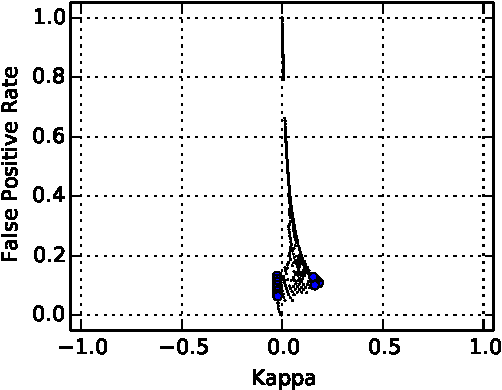
\includegraphics[width=\linewidth]{figs/Kappa-fpr-selected-crop}
        \caption{$\kappa$-$fpr$ diagram}
        \label{fig:MinMax-Kappa-fpr}
    \vspace{0.7cm}
    \end{subfigure}
    \begin{subfigure}[b]{\columnwidth}
        \centering
        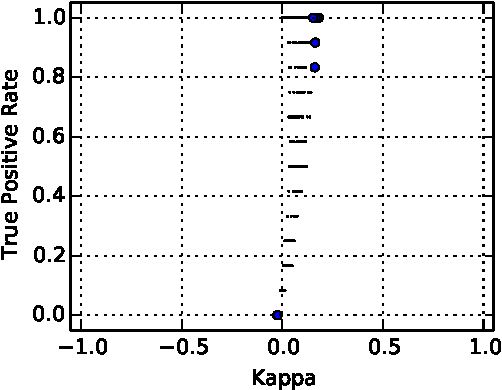
\includegraphics[width=\linewidth]{figs/Kappa-tpr-selected-crop}
        \caption{$\kappa$-$tpr$ diagram}
        \label{fig:MinMax-Kappa-tpr}
    \end{subfigure}
    \caption{Illustration of selected detectors (large blue circles) based on MinMax-Kappa pruning technique. All remaining detectors (small black dots) are pruned.}
    \label{fig:MinMax-Kappa-fpr-tpr}
    \end{adjustbox}
\end{figure}

\begin{figure}[tbh]
    \centering
    \begin{adjustbox}{minipage=\linewidth,scale=0.8}
    \begin{subfigure}[b]{\columnwidth}
        \centering
        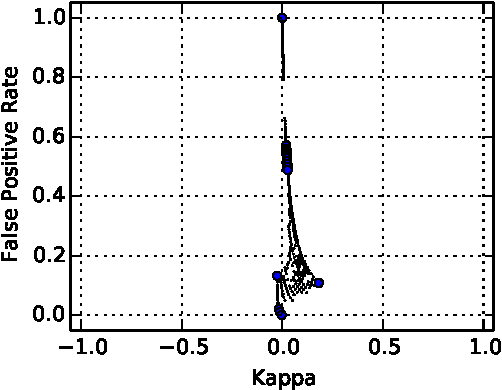
\includegraphics[width=\linewidth]{figs/ROCCH-GT-Kappa-fpr-selected-crop}
        \caption{$\kappa$-$fpr$ diagram}
        \label{fig:ROCCH-Kappa-fpr}
    \vspace{0.7cm}
    \end{subfigure}
    \begin{subfigure}[b]{\columnwidth}
        \centering
        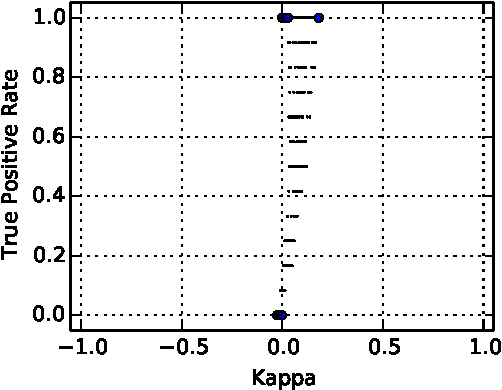
\includegraphics[width=\linewidth]{figs/ROCCH-GT-Kappa-tpr-selected-crop}
        \caption{$\kappa$-$tpr$ diagram}
        \label{fig:ROCCH-Kappa-tpr}
    \end{subfigure}
    \caption{Illustration of selected detectors (large blue circles) based on ROCCH-Kappa pruning technique. All remaining detectors (small black dots) are pruned.}
    \label{fig:ROCCH-Kappa-fpr-tpr}
    \end{adjustbox}
\end{figure}

\begin{figure}[tbh]
    \centering
    \begin{adjustbox}{minipage=\linewidth,scale=0.8}
    \begin{subfigure}[b]{\columnwidth}
        \centering
        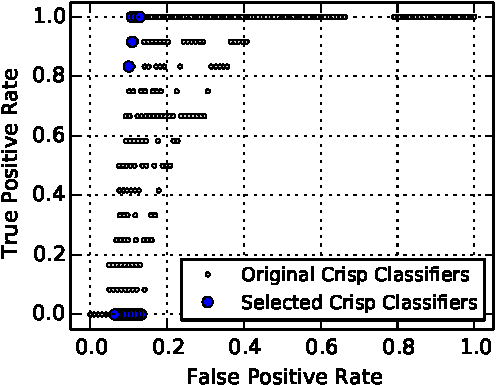
\includegraphics[width=\linewidth]{figs/roc-MinMax-Kappa-selected-crop}
        \caption{MinMax-Kappa pruning}
        \label{fig:ROC-MinMax-Kappa}
    \vspace{0.7cm}
    \end{subfigure}
    \begin{subfigure}[b]{\columnwidth}
        \centering
        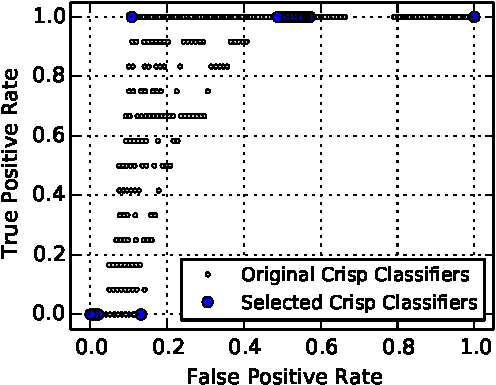
\includegraphics[width=\linewidth]{figs/roc-ROCCH-KAPPA-PairWise-selected-crop}
        \caption{ROCCH-Kappa pruning}
        \label{fig:ROC-ROCCH-Kappa}
    \end{subfigure}
    \caption{Illustration of the selected detectors for combination mapped onto the ROC space (large blue circles). All other detectors (small black dots) can be pruned.}
    \label{fig:ROC-MinMax-vs-ROCCH-Kappa}
    \end{adjustbox}
\end{figure}


\subsection{ROCCH-Kappa Pruning}
\label{sub:rocch-kappa}

This technique also tries to select accurate detectors and then find a set of detectors with complimentary errors.
In contrast with MinMax-Kappa, this technique considers the detectors that are on the facet of the ROCCH in the ROC space.
These detectors are selected since they are the most accurate available detectors that covers the whole range of $fpr$ and $tpr$ trade-off.
The Kappa measure is then used to select diverse detectors with reference to those on ROCCH.
The technique computes the Kappa value of each detector on the ROCCH and all the remaining detectors, sort the resulting values in ascending order.
Detectors with larger values of Kappa are discarded, since they provide similar decisions (or errors) to those provided by the select detectors (on the ROCCH).

The most diverse detectors are those that provide negative or close to zero Kappa values ($\kappa \leq 0$), however are not trivial detectors (providing always either positive or negative decisions).
The only parameter of the ROCCH-Kappa is the number of detectors to be selected for each detector on the ROCCH.
In practice, the number of detectors on the ROCCH is small ([3-20] detectors).
Figure~\ref{fig:ROCCH-Kappa-fpr-tpr} shows an example of the selected detectors from our experiment, according to the ROCCH-Kappa technique, where the Kappa values (on the X-axis) for the selected detectors are plotted against false positive (Figure~\ref{fig:ROCCH-Kappa-fpr}) and true positive  (Figure~\ref{fig:ROCCH-Kappa-tpr}) rates.
Similarly, these selected points (large, blue) are the $\mathcal{C}_{\mbox{selected}}$ in Algorithm~\ref{PBC}, while all remaining detectors (small points) can be pruned.
Figure~\ref{fig:ROC-ROCCH-Kappa} map the detectors selected by ROCCH-Kappa to the ROC space, which could be compared to those selected by MinMax-Kappa in Figure~\ref{fig:ROC-MinMax-Kappa}.

\subsection{MinMax-, ROCCH- Pruning with dCor and dCov}
\label{sub:minmax-rocch-dcov}
These techniques are using the logic we proposed in section~\ref{sub:minmax-kappa} and section~\ref{sub:rocch-kappa}. The novelty behind them is to use newer and stronger distance correlation, which is described in section~\ref{sec:dcov-dcor}. With the help of these two new metrics and integrating them with MinMax and ROCCH techniques; we are more confident in the performance of our PBC method. With this approach the newly proposed PBC method is working well and is stable at all times. More specifically because we use this method with a rational measure of agreement, we can expect to get the reasonable results.

Here in both dCor and dCov; if the result of comparing two different vectors is equal to $0$ indicates that the vectors are surely independent of each other; and if the result is equal to $1$, it means they are exactly similar to each other.

\subsection{Expected Value of Boolean Combination}
\label{sub:expected-value}

Expected Value of Boolean Combination (EVBC)
Our other approach for pruning classifiers is using Expected value. To do that we calculate expected values of combinations of each classier with every other classifiers. This is an iterative method that would be applied on every classifier we have. First we select a classifier, classifier X. To calculate expected value of a combination we need to choose another classifier such as classifier Y from our pool of classifiers. Since we have 10 different Boolean operations we could produce 10 different new classifiers by combining classifier X and Y. Here, we explain our formula for one of the Boolean operation but we could easily extend it for all the rest.

As we explained earlier we could identify each classifier by its TPR-FPR on ROC curve, therefore we want to calculate expected value of TPR-FPR of the new classifier. To calculate TPR and FPR of the combination ($tpr_C, fpr_C$) from Classifier X with ($TPR_X, FPR_X$) and classifier $Y$ with ($TPR_Y, FPR_Y$) we use the equations below:

\begin{multline}
% \begin{equation}
TPR_C = B1 \times TPR_X \times TPR_Y+B2\times TPR_X \times(1- TPR_Y)+\\B3\times(1- TPR_X)\times TPR_Y+B4\times(1- TPR_X)\times(1- TPR_Y)
% \end{equation}
\end{multline}

\begin{multline}
% \begin{equation}
FPR_C = B1 \times FPR_X \times FPR_Y+B2\times FPR_X \times(1- FPR_Y)+\\B3\times(1-FPR_X)\times FPR_Y+B4\times(1- FPR_X)\times(1-FPR_Y))
% \end{equation}
\end{multline}


Which B1, B2, B3, B4 is binary representation of our Boolean operation (And = '1000', OR = '1110', XOR = '0110', etc. )
For example for XOR we would have:

\begin{multline}
% \begin{equation}
TPR_C = 0 \times TPR_X \times TPR_Y+1\times TPR_X \times(1- TPR_Y)+\\1\times(1- TPR_X)\times TPR_Y+0\times(1- TPR_X)\times(1- TPR_Y)
% \end{equation}
\end{multline}

\begin{multline}
% \begin{equation}
FPR_C = 0 \times FPR_X \times FPR_Y+1\times FPR_X \times(1- FPR_Y)+\\1\times(1-FPR_X)\times FPR_Y+0\times(1- FPR_X)\times(1-FPR_Y))
% \end{equation}
\end{multline}

Now we have 3 classifiers X, Y and the combination of them using XOR operation (Classifier C) as it's shown in the picture below. Now we need to evaluate the goodness of classifier C compared to X and Y. Area Under the Curve (AUC) is a function, which can be used to evaluate the goodness. Based on the coordination of each classifier on ROC curve we can compute AUC of the classifier with the following formula:


\begin{figure}[H]
\centering
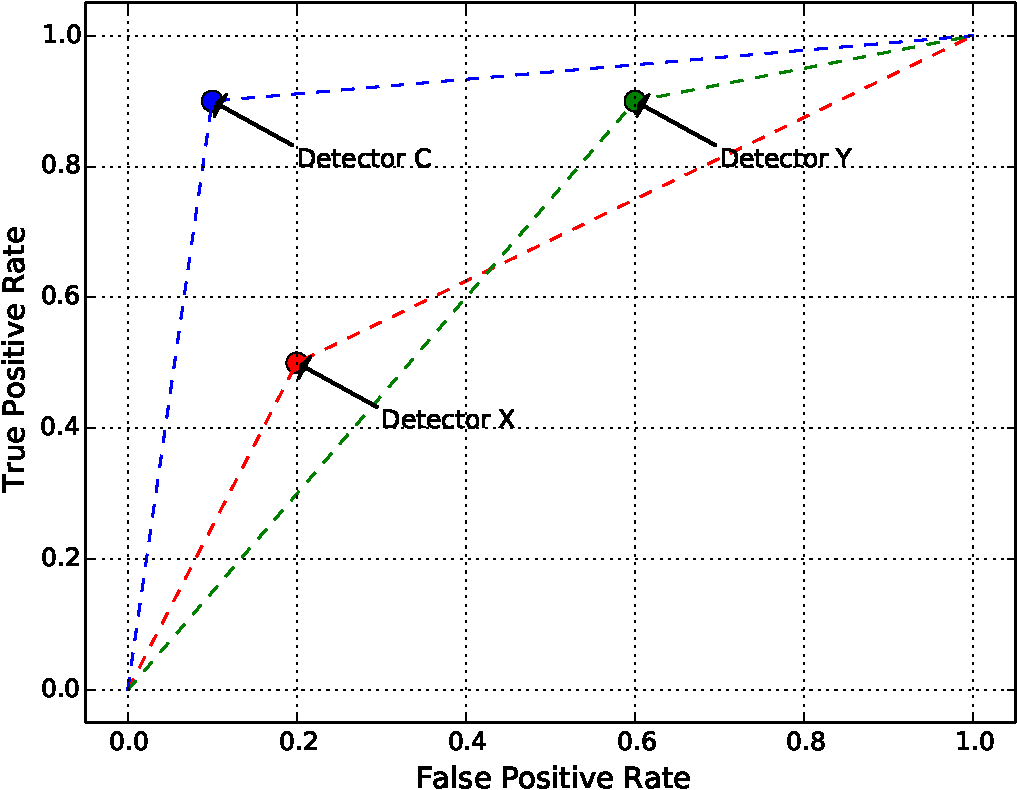
\includegraphics[scale=0.75]{figs/Classifiers_X_Y_C}
\caption{Combination of classifier X and Y lead to C}
\label{fig::X_Y_C}
\end{figure}


We compute AUC for classifier X, Y and C and keep classifier C only if its AUC is greater than AUC of both classifiers X and Y. Greater AUC means that our classifier is much closer to the ground truth (which will give us the TPR = 1 and FPR = 0).
If AUC$_C$ is greater than AUC$_X$ and AUC$_Y$ we keep the difference in AUC as the improvement of that classifier with the specific Boolean operation used. The variable that keeps the improvement for classifier X is IMP as defined below:
$IMP_X  = AUC_C - Max(AUC_X, AUC_Y)$
We calculate $IMP_X$ for all 10 Boolean operations and add them to the previous value. At the end, $IMP_X$ has the expected value of all of the combination possible between classifiers X and Y using 10 Boolean operations. We repeat these steps for classifier X in combination with the rest of classifiers, choosing one each time as a new classifier Y and update $IMP_X$. The final $IMP_X$ value has the total expected value of the improvement with respect to all the combinations if we select classifier X. After we compute $IMP_X$ for classifier X and the rest of classifiers we will update the value in our table in a $TPR_X$ $FPR_X$ position with $IMP_X$. We repeat all these steps for every classifier we have and update their IMP in the table and then we can create a table shown below with each cell representing the expected value of the classifier combinations getting improved. We select that classifier with the most improvement.

\begin{figure}[H]
\centering
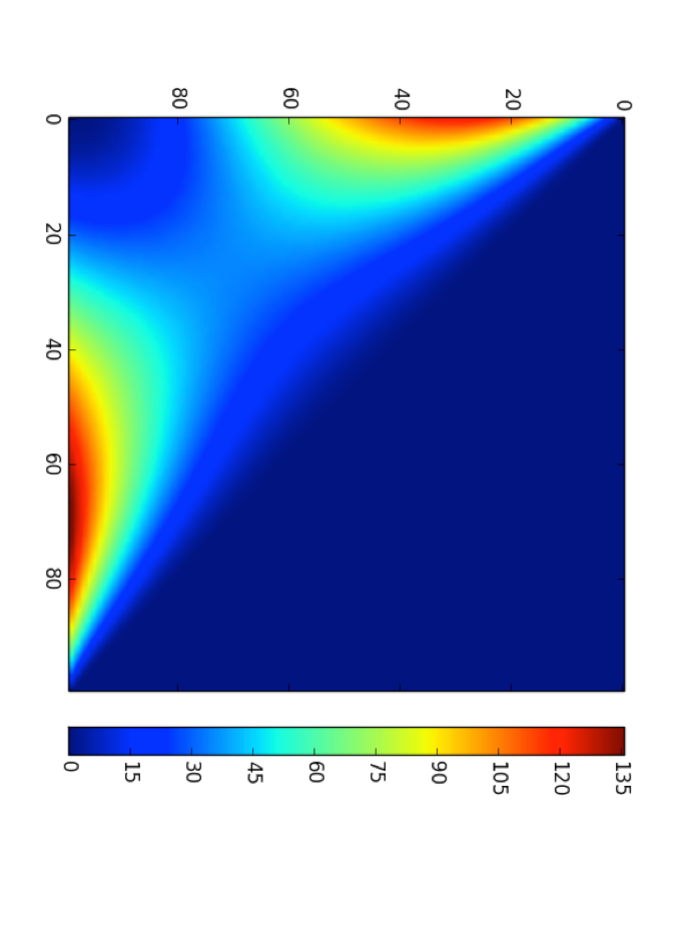
\includegraphics[scale=1]{figs/expected_value}
\caption{expected value of all classifiers in the ROC space}
\label{fig::expected_value}
\end{figure}

As shown in Figure~\ref{fig::expected_value}  the representation of that table if we use color plotting. The red region shows classifiers with higher IMP and the blue region shows classifier with low IMP. That means if we select our basket of classifiers from red region we would have a higher chance to get better classifiers after combination of those pruned classifiers. Our assumption for creating above table was that we have all the possible classifiers with 2 digits precision and after computing all possible combination for all the classifiers we set the value of each cell below minor diameter to zero (all the classifiers below random line) since want to evaluate goodness of classifiers better than random guess.
We can re-produce the same table by computing the expected value of combination just for the classifiers that already we have; by doing that we will get the below table (plot) and we can prune our classifier based on this new table.

\section{Complexity Analysis}
\label{sub:complexity}

Given $K$ soft detectors, let $n_i$ be the number of decision thresholds or crisp detectors produced by each of the soft detector $D_i$, $i=1,\ldots, K$, on the validation set $\mathcal{V}$.
Let $n=\sum_{i=1}^{K} n_i$ the total number of crisp detectors in the ensembles, and $n_{avg} = n/K$ the average number of crisp detectors produced by soft detectors.

A brute-force search for optimal combination is infeasible in practice due to the doubly exponential combinations.
In fact, for $n$ crisp detectors there are $2^n$ possible outcomes that can be combined in $2^{2^n}$ ways, which makes the brute-force combination impractical even for small $n$ values \cite{Barreno2008}.
Even only pairwise combination of $n$ crisp detectors, which requires $\mathcal{O}(n^2)$ Boolean operations, may not be feasible in practise for large $n$ values.
The sequential combination of the IBC algorithm reduces its worst-case time complexity to $\mathcal{O}(n_{avg}^2 + Kn_{avg})$ Boolean operations.

Both pruning techniques are capable of reducing the size of the selected subset of detectors (for Boolean combination) up to a user defined maximum number ($U$).
The worst-case time complexity required by MinMax-Kappa technique to select $U$ crisp detectors (and prune the rest) is $\mathcal{O}(n(\log n + 1) + U^2)$.
It requires about $n(\log n + 1)$ operations for computing and sorting the Kappa values for all crisp detectors, and $U^2$ for the pairwise Boolean combinations of the $U$ retained detectors.
For ROCCH-Kappa technique however the worst-case time complexity is of the order $\mathcal{O}(n(\log n +n_{ev}) + U^2)$, where $n_{ev}$ is the number of emerging vertices which is typically around ten.
The additional $n_{ev}$ factor is due to the computation of Kappa is repeated $n_{ev}$ times for each emerging point on the ROCCH.
For numerical comparison, Table~\ref{tab:time-complexity} shows the average time for each combination and pruning technique used in our experiments.


\chapter{Experiment and Results} \label{chapter4}

\section{Experiments on System Call Data set}
\label{sec:experiments}

We evaluate the accuracy and efficiency of our pruning techniques using a modern system call data set, called ADFA Linux Data set (ADFA-LD), which has been recently made publicly available on the website of the University of New South Wales \cite{Creech2013a}.
The ADFA-LD data set is generated by exploiting various security vulnerabilities in a Ubuntu operating system (OS) hosting a web server.
The systems consists of a fully patched Ubuntu Linux 11.04 OS with an Apache 2.2.17 web server, PHP 5.3.5 server side scripting engine, TikiWiki 8.1 content management system, FTP server, MySQL 14.14 database management system and an SSH server.
First they collect normal system call traces by letting users perform basic operations, such as web browsing and Latex document preparations under controlled situations.
The anomalous system call traces are collected while the system is being under six types of attack vectors resulting in a total of 60 attacks.
These attacks were launched by a certified penetration tester against the system and included web-based exploitation, simulated social engineering, poisoned executable, remotely triggered vulnerabilities, remote password brute-force attacks and system manipulation.
The authors of the ADFA-LD have organized the data set into 833 normal traces for training the anomaly detectors, and 4373 normal traces and 60 anomalous traces for testing.

In our experiments, we used the following experimental setup.
First, we trained 20 HMMs with different numbers of states (i.e., $K=20$ soft detectors), using the 833 normal traces provided for training in the ADFA-LD data set.
On average, the output of each HMM is thresholded into $n_{avg} = 100$ thresholds or crisp detectors, which provides $n = K \times n_{avg} = 20\times 100 =2000$ crisp detectors in the ensemble.

The objective is to choose the most accurate subset from this ensemble for combination while pruning the remaining detectors according to our MinMax-Kappa or ROCCH-Kappa technique.
Then, the ROC curves and AUC results are compared to those of IBC and the pairwise brute-force Boolean Crisp combination (BBC2).
BBC2 is another baseline, which is the PBC Algorithm~\ref{PBC}, but without any pruning mechanism.

For evaluation of performance, a 5-fold cross-validation (5FCV) is applied to the test set comprising the 4373 normal and the 60 anomalous traces.
Since the number of anomalous traces is relatively small with reference to the normal ones, we applied the cross validation to partition the normal and anomalous sets separately, such that we keep the same ratio (normal to anomalous) and guarantee that all folds include the anomalies.
Accordingly, each fold contains 874 traces selected at random from the 4373 normal traces and 12 attacks traces selected at random from the 60 attack traces.

In contrast with the standard way of applying the 5FCV, we used one fold for computing the Boolean combination according to each of the combination technique,
and the remaining four folds (i.e., 3498 normal traces and 48 attack traces) are used for evaluating and benchmarking the detection performance.
This is because we wanted to test the boost in performance while using a small number of anomalies during combination. The results are shown in section~\ref{sec:results-ADFA}.

For the second data set, we used the Canali data set~\cite{Canali2012}. The data was generated from 10 different machines. Our models, which are 4 HMMs and 5 SVMs, are trained on the normal data from: anubis-good + machine1 + ... + machine9, and the scores that we used are computed on the test data: machine10 that consist of (23 normal traces) + malware (5855 anomalous traces).

With this data set, in contrast with ADFA that we showed the boost in result with a small number of anomalies we want to show even when  anomalies are the majority of the test set with PBC technique there is a boost in result.
Here again we applied the PBC technique with help of different distance correlation metric (Kappa, Distance Covariance, Distance Correlation) and compare the result with BBC2 and IBC. For Canali we used 5FCV approach as well. The result are shown in section~\ref{sec:results-canali}.



\section{Results (ADFA)}
\label{sec:results-ADFA}



\begin{figure}[t]
\centering
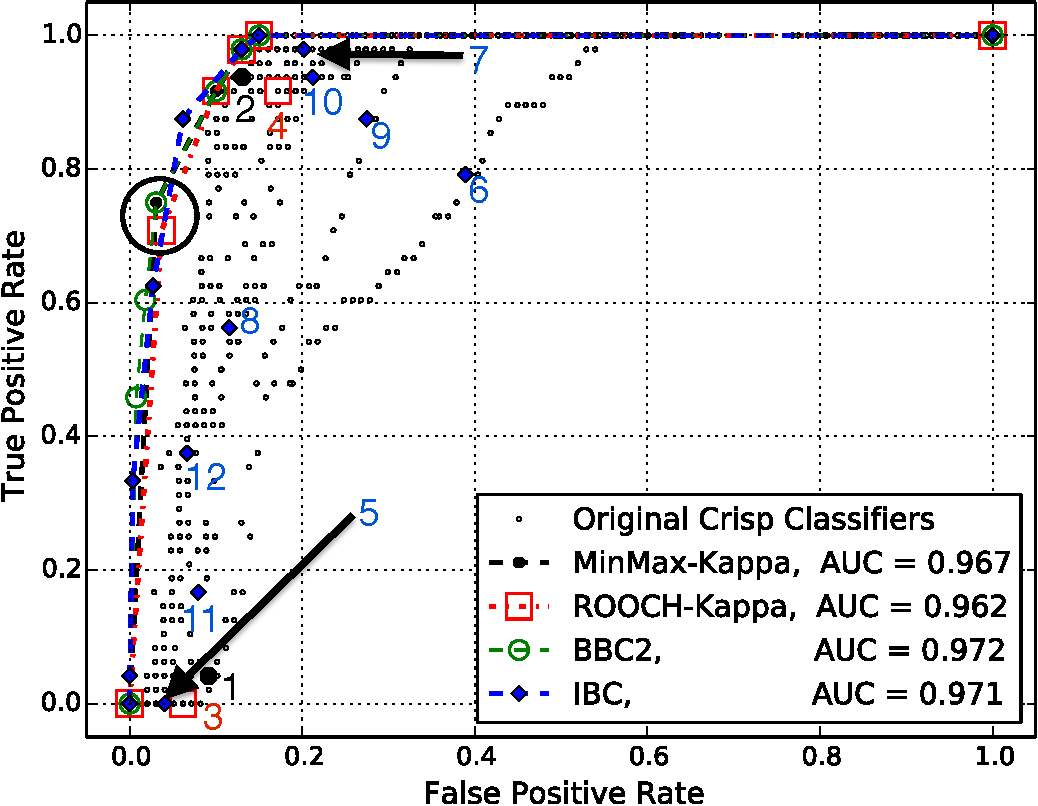
\includegraphics[width=\columnwidth]{figs/roc_curves_testing_fold3}
\caption{One of the ROC curves results of 5-folds cross-validation of Boolean combination on one fold and evaluated on four folds. The numbers represent the crisp detectors selected for combination (by each technique) to achieve about the same operational point as denoted by the large black circle}
\label{fig:roc_curves}
\end{figure}

\begin{figure}[t]
\centering
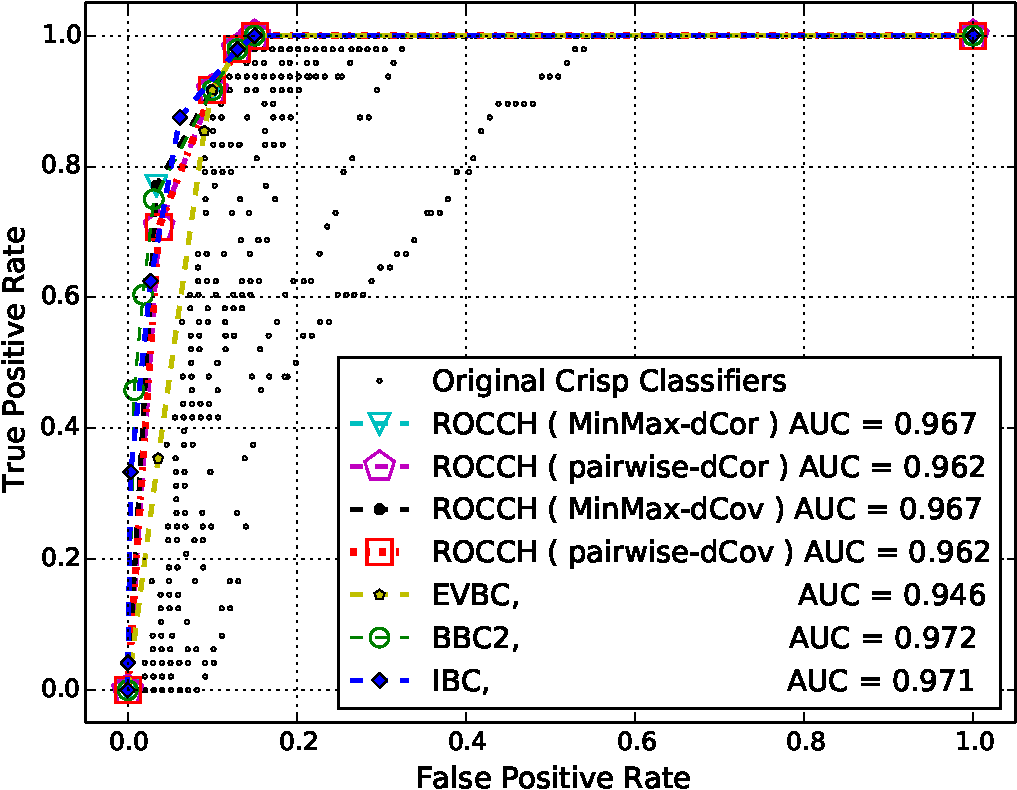
\includegraphics[scale=0.85]{figs/ADFA-dcov/IBC_BCC_Pruned_Classifier_ConvexHull_withoutRandom_validation}
\caption{The same ROC curves results of 5-folds cross-validation of Boolean combination on one fold and evaluated on four folds that was used in Figure~\ref{fig:roc_curves} with other distance correlation metrics}
\label{fig:roc_curves_dcov}
\end{figure}



\begin{table}[b]
    \centering
    \renewcommand{\arraystretch}{1.3}
    \caption{Average AUC values and their standard deviations over the 5FCV for each techniques. Design on one fold and evaluated on four folds. }
    \label{tab:auc}
    \centering
    \scalebox{1.2}{
    \begin{tabular}{lrr}
        \hline
        Method Name & Mean & Std\\
        \hline
        \hline
        BBC2 & 0.97426 & 0.001  \\
        IBC & 0.97276 & 0.001  \\
        MinMax-Kappa & 0.97074 & 0.003  \\
        ROCCH-Kappa & 0.97051 & 0.003  \\
        EVBC & 0.94472 & 0  \\
        MinMax-dCor & 0.9673 & 0.006  \\
        ROCCH-dCor &  0.97067 & 0.005 \\
        MinMax-dCov & 0.96515 & 0.004  \\
        ROCCH-dCov &  0.97051 & 0.005  \\
        \hline
    \end{tabular}}
\end{table}

\begin{table}[b]
    % \normalsize
    \small
    \centering
    \renewcommand{\arraystretch}{1.3}
    \caption{Comparison of pruning and combination time (seconds) and number of Boolean operations required to achieve the final ROCCH during the design phase, and the number of selected detectors during the operational phase. All values are averaged over 5FCV.}
    \label{tab:time-complexity}
    \centering
    \scalebox{1}{
    \begin{tabular}{lrrr|r}
    % \begin{tabular}{L{1.8cm}rrr|r}
        & \multicolumn{3}{c}{\bf Design Phase } & \bf Operations \\
        \cline{2-5}
        Method &   Pruning &  Combination &  \# Boolean &  \# Combined\\
        Name &     Time    &  Time &  operations & detectors\\
        \hline
        \hline
        BBC2            & N/A     & 16364 &   $4,000,000$ & 2\\ %1617
        IBC             & N/A     & 11    &   $11,000$  & 11 \\
        MinMax-Kappa    & 1.6   & 15    &   $19,701$    & 2\\
        ROCCH-Kappa     & 11.8  & 38    &  $37,701$     & 2 \\
        EVBC     & 370  &   13  &  $...$     & 2 \\
        MinMax-dCor    &   74 &   16  &   $19,701$    & 2\\
        ROCCH-dCor     & 190  &   30  &  $37,701$     & 2 \\
        MinMax-dCov    &   64 &    17 &   $19,701$    & 2\\
        ROCCH-dCov     & 185  &    37 &  $37,701$     & 2 \\
        \hline
    \end{tabular} }
\end{table}


Figure~\ref{fig:roc_curves} shows the ROC curves and the AUC performance for both pruning techniques proposed in this paper (MinMax- and ROCCH-Kappa) compared to those of IBC and BBC2 (PBC with no pruning mechanism). And Figure~\ref{fig:roc_curves_dcov} shows the same ROC (the same fold) for both MinMax- and ROCCH- technique with different distance correlation as discussed in section~\ref{sub:minmax-rocch-dcov}.

These results are for one of the 5FCV experiments (the combinations are computed on one fold and evaluated on four) as described in Section~\ref{sec:experiments}.
As shown in the figure the results are comparable both in term of AUC values and the shape of the ROC curves.
This is also confirmed in Table~\ref{tab:auc}, where the AUC values of each combination technique is averaged over the 5FCV experiments.

Table~\ref{tab:time-complexity} shows the average over the 5FCV of the  pruning time (for MinMax-Kappa,  ROCCH-Kappa, MinMax-dCor, MinMax-dCov, ROCCH-dCor, ROCCH-dCov), combination time, and number of Boolean operations required by each technique to achieve the final ROCCH (as shown in  Figure~\ref{fig:roc_curves} and  Figure~\ref{fig:roc_curves_dcov} for one fold).  

We set the maximum number of selected detectors to $U=50$ for all the above-mentioned techniques (this can be further optimized, but gave good trade-off between performance and time complexity).
Therefore, the input to these pruning techniques is $n=2000$ crisp detectors, while the output is a subset of a maximum size of $50$ detectors provided for Boolean combination (in PBC Algorithm).
MinMax-Kappa took about $1.6$ seconds in average to select the best subset, while ROCCH-Kappa took about ten times more due the $n_{ev}$ factor, which is described in Section~\ref{sub:complexity}, to prune the ensemble of $n=2000$ detectors.
Furthermore, MinMax-Kappa is able to select a smaller number of detectors than $U=50$ on average and computes the Kappa values once, which explains the reduction in combination time and number of Boolean operations compared to those of ROCCH-Kappa, as shown in Table~\ref{tab:time-complexity}.
Thereby, although both techniques provide similar AUC performance, MinMax-Kappa is slightly preferred due to its improved efficiency  compared to ROCCH-Kappa.

Table~\ref{tab:time-complexity} also shows that our MinMax-Kappa techniques was able to achieve the same AUC performance of BBC2 (the pairwise Boolean combination of the $2000$ detectors), by selecting less than $50$ detectors out of the $2000$ ones.
More interestingly, MinMax-Kappa achieved these results with an average time of three magnitudes lower than that of BBC2, and about 200 times fewer Boolean operations.

Compared to IBC, MinMax-Kappa requires, on average, slightly more combination time and a larger number of Boolean operations to achieve the same AUC performance.
However, the number of selected detectors and Boolean functions required to realize each vertex on the ROCCH is on average five times more according to our experiments.
For instance, to achieve the final operating points denoted with a  large black circle on Figure~\ref{fig:roc_curves}, MinMax-Kappa uses two detectors and one Boolean function according to the following formula:
\begin{equation*}
    \neg D_1 \oplus  D_2
\end{equation*}
Note that in Figure~\ref{fig:roc_curves}, we only shown the number of crisp detectors not to clutter the figures (i.e., 1 means $D_1$)
\\
Similarly, ROCCH-Kappa uses the following detectors and Boolean function to achieve similar operating point:
\begin{equation*}
    \neg D_3 \oplus  D_4
\end{equation*}
However to achieve similar point of operations, IBC requires eight detectors combined according to the following Boolean operations:
\begin{equation*}
    (((((((D_5 \oplus D_6) \land \neg D_{11})  \land D_7) \oplus D_8) \equiv D_9) \lor D_{10})  \land D_{12})
\end{equation*}

The average number of combined detectors on the final ROCCH over the 5FCV is about 10 detectors when using IBC compared to two detectors when using PBC with MinMax-Kappa pruning as shown in the last column of Table~\ref{tab:time-complexity}.
This sequence of combination rules grows linearly with the number of soft detector $K$, which makes IBC results difficult to analyse and understand for large $K$ values.
In contrast to IBC, the combination of two detectors according to combination of PBC with MinMax-Kappa are insensitive to order in which detectors are input to the algorithm, which makes the search for the best subset of detectors easier.
However, MinMax-Kappa requires an optimization of the maximum number of detectors $U$ that trades off the complexity and the accuracy.
Setting an ADS based on two HMMs into operations, requires less time and memory resources to provide the output probabilities of the input system call sequences.
In addition, operating a small number of detectors becomes critical in application of anomaly detection mobile security, due to the constraint on power resources.

%%%%%%%%%%%%%%%%%%%%%%%%%% 4 Folds results

\begin{figure}[t]
\centering
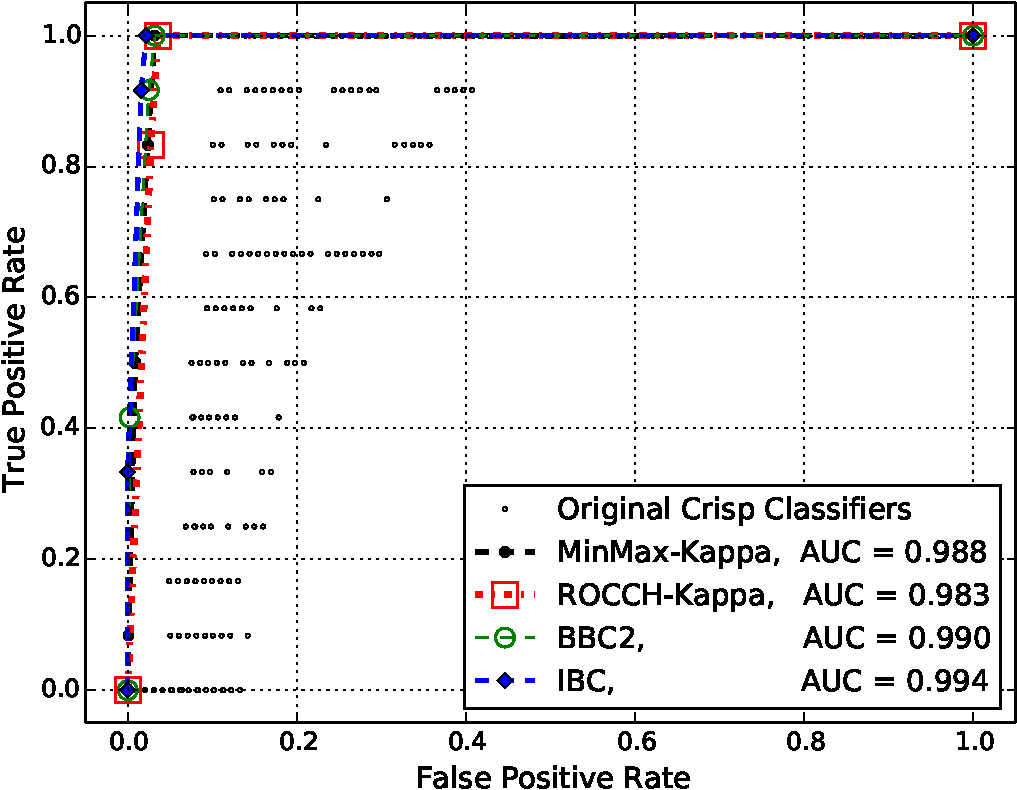
\includegraphics[width=\columnwidth]{figs/roc_curves_training_on_4_folds_testing_on_1-crop}
\caption{One of the ROC curves results of 5-folds cross-validation of Boolean combination on four folds and evaluated on one fold.}
\label{fig:roc_curves4}
\end{figure}

\begin{figure}[t]
\centering
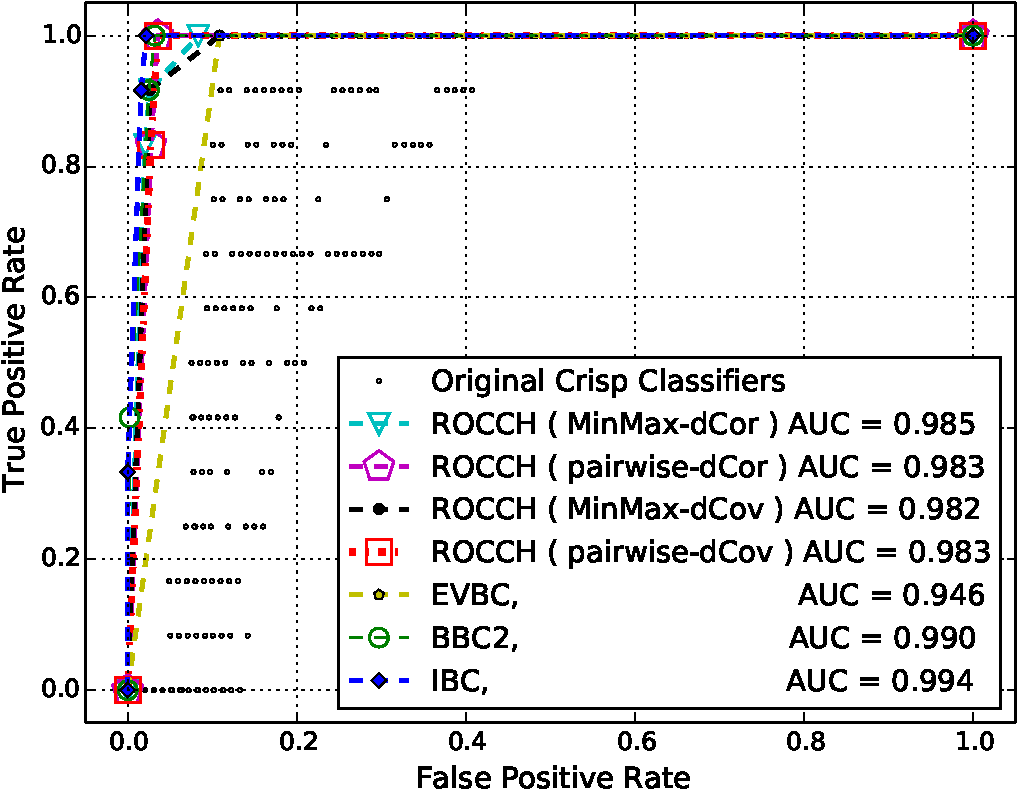
\includegraphics[width=\columnwidth]{figs/ADFA-dcov/IBC_BCC_Pruned_Classifier_ConvexHull_withoutRandom_validation_4fold}
\caption{The same ROC curves results of 5-folds cross-validation of Boolean combination on four folds and evaluated on one fold that was used in fig.~\ref{fig:roc_curves4} with other distance correlation metrics.}
\label{fig:roc_curves4_dcov}
\end{figure}




\begin{table}[b]
    \centering
    \renewcommand{\arraystretch}{1.3}
    \caption{Average AUC values and their standard deviations over the 5FCV for each techniques. Design on four folds and evaluated on one fold.  }
    \label{tab:auc4}
    \centering
    \scalebox{1.2}{
    \begin{tabular}{lrr}
        \hline
        Method Name & Mean & Std\\
        \hline
        \hline
        BBC2 & 0.98177 & 0.00636  \\
        IBC & 0.98003 & 0.01127  \\
        MinMax-Kappa & 0.97806 & 0.00640  \\
        ROCCH-Kappa & 0.97578 & 0.00585  \\
        EVBC & 0.94472 & 0  \\
        MinMax-dCor & 0.9725 & 0.012  \\
        ROCCH-dCor &  0.9752 & 0.005 \\
        MinMax-dCov & 0.96268 & 0.011  \\
        ROCCH-dCov &  0.9753 & 0.005  \\
        \hline
    \end{tabular}}
\end{table}

We conducted an alternative case study to check the impact on ROC and AUC performance of all Boolean techniques, when the number of anomalies is increased during the design phase.
Therefore, instead of using one fold (comprising $12$ attack traces and $874$ normal traces) for selecting the crisp detectors and the corresponding Boolean functions, as described in Section~\ref{sec:experiments}, we used 4 folds ($48$ attack traces and $3498$ normal traces) and one fold for evaluation of performance.

Figure~\ref{fig:roc_curves4} and figure~\ref{fig:roc_curves4_dcov} show the ROC curves and the AUC performance for all techniques, PBC with MinMax-Kappa, ROCCH-Kappa, MinMax-dCor, MinMax-dCov, ROCCH-dCor, ROCCH-dCov, IBC and BBC2.
Again, the presented results are for one of the 5FCV experiments (but the combinations are computed on four folds and evaluated on one).
As shown in the figure, all techniques provide comparable results; however, with a large improvement in detection accuracy over those presented in Figure~\ref{fig:roc_curves}.
For instance, for detecting all attacks ($tpr = 100\%$) the false positive rate is now $fpr\approx  2\%$ compared to $fpr\approx 16\%$ in Figure~\ref{fig:roc_curves}.
This boost in performance can be also seen in Table~\ref{tab:auc4} in terms of average AUC values for each combination technique over the 5FCV experiments.
The results of this experiments show, as expected, that when the system is provided with more normal or attack traces, the overall performance of all Boolean combination techniques improves.
In such cases, there is no need to retrain the original detectors (HMMs in our case), which is a time consuming process, but the design phase of Boolean combination techniques must be repeated.
This provides an advantage for IBC and PBC, since they are efficient in selecting the detectors for final operations.
However, our PBC approach will always provide two detectors for each emerging point on the ROCCH, which is less costly to operate and easier to analyse in real-world setting.

\section{Results (Canali)}
\label{sec:results-canali}

\begin{figure}[t]
\centering
\includegraphics[width=\columnwidth]{figs/Canali/IBC_BCC_Pruned_Classifier_ConvexHull_withoutRandom_validation_4fold_kappa}
\caption{One of the ROC curves results of 5-folds cross-validation of Boolean combination on four folds and evaluated on one fold on Canali.}
\label{fig:roc_curves_canali}
\end{figure}

\begin{figure}[t]
\centering
\includegraphics[width=\columnwidth]{figs/Canali/IBC_BCC_Pruned_Classifier_ConvexHull_withoutRandom_validation_4fold_dCov}
\caption{The same ROC curves results of 5-folds cross-validation of Boolean combination on one fold and evaluated on four folds that was used in Figure~\ref{fig:roc_curves_canali} with other distance correlation metrics}
\label{fig:roc_curves_dcov_canali}
\end{figure}



\begin{table}[b]
    \centering
    \renewcommand{\arraystretch}{1.3}
    \caption{Average AUC values and their standard deviations over the 5FCV for each techniques. Design on four folds and evaluated on one fold on Canali. }
    \label{tab:auc_canali}
    \centering
    \scalebox{1.2}{
    \begin{tabular}{lrr}
        \hline
        Method Name & Mean & Std\\
        \hline
        \hline
        BBC2 & 0.97398 & 0.008  \\
        IBC & 0.97141 & 0.006  \\
        MinMax-Kappa & 0.95884 & 0.005  \\
        ROCCH-Kappa & 0.9716 & 0.008  \\
        EVBC & 0.95074 & 0.006  \\
        MinMax-dCor & 0.95426 & 0.006  \\
        ROCCH-dCor &  0.96451 & 0.006 \\
        MinMax-dCov & 0.9616 & 0.011  \\
        ROCCH-dCov &  0.96451 & 0.006  \\
        \hline
    \end{tabular}}
\end{table}

Figure~\ref{fig:roc_curves_canali} shows the ROC curves and the AUC performance for both pruning techniques proposed in this paper (MinMax- and ROCCH-Kappa) compared to those of IBC and BBC2 (PBC with no pruning mechanism). They are all applied on Canali data set in order to confirm the consistency of PBC technique regardless of the data set. Figure~\ref{fig:roc_curves_dcov_canali} demonstrates the same ROC (the same fold) for both MinMax- and ROCCH- technique with different distance correlation as discussed in section~\ref{sub:minmax-rocch-dcov}.

These results belong to one of the 5FCV experiments (the combinations are computed on one fold and evaluated on four) as described in Section~\ref{sec:experiments}.
As shown in this figure the results are comparable both in terms of AUC values and the shape of the ROC curves.
This is also confirmed in Table~\ref{tab:auc_canali}, where the AUC values of each combination technique are averaged over the 5FCV experiments.

In this experiment;we set the maximum number of selected detectors to $U = 50$ for all of the above-mentioned techniques similar to what we did for ADFA~\ref{sec:results-ADFA}.
Therefore, the inputs to these pruning techniques are $n=900$ crisp detectors (4 different HMMS and 5 SVMs each thresholded 100 times), while the output is a subset of a maximum size of $50$ detectors provided for Boolean combination (in PBC Algorithm).

Compared to ADFA's result in ~\ref{sec:results-ADFA} here we can see that ROCCH-Kappa generates even better results than IBC, however the difference is not significant yet it persuade us more to use PBC; Since by using PBC we are guaranteed that our final formula is shorter and we have much fewer number of combinations that leads to less calculation time which saves CPU cycles (and get the result very much faster).

Running PBC as discussed in section~\ref{sec:pbc} with completely new data set such as Canali (which is for Windows) and getting promising result is a proof that PBC technique is applicable on various data sets as long as having a diverse detectors trained on the them.

The key for PBC to work well is to have as many diverse detectors as possible.

And therefore the complexity of the detectors is not a determining factor and we only need to keep the diversity of the pool of detectors high. With the help of PBC we prune the pool to create the basket of detectors for combination. In conclusion, PBC with reasonable distance correlation tries to select few samples from each set of detectors such that it represents the original pool.

\section{Threats to Validity}
\label{sec:threat-validity}

A threat to internal validity exists in the implementation of the IBC, BBC2 and PBC algorithms as well as in conducting the experiments for anomaly detection.
We have mitigated this threat by manually verifying the outputs.

We have conducted experiments using only one system call data set derived from the Linux operating system, which consists a threat to external validity of this study.
More experiments are therefore required to generalize the presented results to other data sets, operating systems and other software vulnerabilities.

Evasion attacks could also pose a threat to validity.
For instance, \textit{mimicry} attacks try to mimic the normal system behavior will go undetected with the ADSs that are based on individual system calls or their temporal order \cite{Wagner2002}.
Mimicry attacks could be conducted by an attacker who is able to launch his attack without tempering the normal order of system calls by, for instance, replacing foreign system call sequences (which can be easily detected) with normal ones or by using system call arguments  \cite{Wagner2002}.

The manifestations of such mimicry attacks could be detected by including additional features, such as system call arguments \cite{Bhatkar2006}, return values extracted from the call stack information \cite{Feng2003}, and the user identity \cite{Larson2009}.
An added advantage of multiple detector systems, combined without our PBC, is that they can combine different detectors trained on various features, such as system call arguments, return values and other information flow features to help mitigating such evasion attacks.

\chapter{Conclusion} \label{chapter5}
In this thesis, we proposed PBC, an efficient approach for selecting and combining anomaly detectors, which relies on two novel pruning techniques.

During the design phase, the PBC is able to select a small subset of diverse and accurate detectors for Boolean combinations, while discarding the remaining ones.
The pruning techniques we developed at the core of PBC rely on Kappa measure (MinMax-Kappa) and on the ROC convex hull (ROCCH-Kappa) to aggressively prune redundant and trivial detectors.

The results on ADFA-LD system call data sets show that PBC with both pruning techniques are capable of maintaining similar overall accuracy as measured by the ROC curves to that of IBC and BBC2.
Therefore, our proposed PBC-based ADS is able to prune and combine large number of detectors without suffering from the exponential explosion in number of combinations provided with the pairwise brute-force Boolean combination techniques.
This has been shown analytically (in the time complexity analysis) and confirmed in the experimental results.

During the operational phase, PBC with both pruning techniques always provides two crisp detectors for each combination, while IBC requires an average of $11$ detectors to achieve the same operating point (in terms of true and false positive rates).
The proposed PBC approach is also general and can be applied to combine any soft or crisp detectors or two-class classifiers in a wide range of applications that requires combination of decisions.

Future work involves conducting more experiments using different real-world data sets.
Another interesting direction is to investigate the potential improvement by re-combining the resulting combinations with the selected detectors, and explore other measures of diversity. We also intend to implement the new techniques in TotalADS \cite{Murtaza2014}, a tool we have developed to support multiple anomaly detectors. Finally, we need to investigate how we can reduce the size of traces to enable better scalability. Example of trace abstraction techniques are presented in \cite{Hamou-Lhadj2005,Murtaza2013}.
%\appendix
%\include{appendix1}
%\codebaselineskip
%\cumakebibliography{IEEEabrv,MyRef}
%\theendnotes

\bibliographystyle{ieeetr}%IEEEtrans
\bibliography{Soudi2015}


\end{document}